% **************************************************************************************************************
% A Classic Thesis Style
% An Homage to The Elements of Typographic Style
%
% Copyright (C) 2015 André Miede http://www.miede.de
%
% If you like the style then I would appreciate a postcard. My address 
% can be found in the file ClassicThesis.pdf. A collection of the 
% postcards I received so far is available online at 
% http://postcards.miede.de
%
% License:
% This program is free software; you can redistribute it and/or modify
% it under the terms of the GNU General Public License as published by
% the Free Software Foundation; either version 2 of the License, or
% (at your option) any later version.
%
% This program is distributed in the hope that it will be useful,
% but WITHOUT ANY WARRANTY; without even the implied warranty of
% MERCHANTABILITY or FITNESS FOR A PARTICULAR PURPOSE.  See the
% GNU General Public License for more details.
%
% You should have received a copy of the GNU General Public License
% along with this program; see the file COPYING.  If not, write to
% the Free Software Foundation, Inc., 59 Temple Place - Suite 330,
% Boston, MA 02111-1307, USA.
%
% **************************************************************************************************************
\RequirePackage{fix-cm} % fix some latex issues see: http://texdoc.net/texmf-dist/doc/latex/base/fixltx2e.pdf
\documentclass[ twoside,openright,titlepage,numbers=noenddot,headinclude,%1headlines,% letterpaper a4paper
                footinclude=true,cleardoublepage=empty,abstractoff, % <--- obsolete, remove (todo)
                BCOR=5mm,paper=a4,fontsize=11pt,%11pt,a4paper,%
                ngerman,american,%
                ]{scrreprt}

%********************************************************************
% Note: Make all your adjustments in here
%*******************************************************
% ****************************************************************************************************
% classicthesis-config.tex 
% formerly known as loadpackages.sty, classicthesis-ldpkg.sty, and classicthesis-preamble.sty 
% Use it at the beginning of your ClassicThesis.tex, or as a LaTeX Preamble 
% in your ClassicThesis.{tex,lyx} with % ****************************************************************************************************
% classicthesis-config.tex 
% formerly known as loadpackages.sty, classicthesis-ldpkg.sty, and classicthesis-preamble.sty 
% Use it at the beginning of your ClassicThesis.tex, or as a LaTeX Preamble 
% in your ClassicThesis.{tex,lyx} with % ****************************************************************************************************
% classicthesis-config.tex 
% formerly known as loadpackages.sty, classicthesis-ldpkg.sty, and classicthesis-preamble.sty 
% Use it at the beginning of your ClassicThesis.tex, or as a LaTeX Preamble 
% in your ClassicThesis.{tex,lyx} with \input{classicthesis-config}
% ****************************************************************************************************  
% If you like the classicthesis, then I would appreciate a postcard. 
% My address can be found in the file ClassicThesis.pdf. A collection 
% of the postcards I received so far is available online at 
% http://postcards.miede.de
% ****************************************************************************************************


% ****************************************************************************************************
% 0. Set the encoding of your files. UTF-8 is the only sensible encoding nowadays. If you can't read
% äöüßáéçèê∂åëæƒÏ€ then change the encoding setting in your editor, not the line below. If your editor
% does not support utf8 use another editor!
% ****************************************************************************************************
\PassOptionsToPackage{utf8}{inputenc}
	\usepackage{inputenc}

% ****************************************************************************************************
% 1. Configure classicthesis for your needs here, e.g., remove "drafting" below 
% in order to deactivate the time-stamp on the pages
% ****************************************************************************************************
\PassOptionsToPackage{eulerchapternumbers,listings,%drafting,%
					 pdfspacing,%floatperchapter,%linedheaders,%
					 subfig,beramono,eulermath,parts}{classicthesis}                                        
% ********************************************************************
% Available options for classicthesis.sty 
% (see ClassicThesis.pdf for more information):
% drafting
% parts nochapters linedheaders
% eulerchapternumbers beramono eulermath pdfspacing minionprospacing
% tocaligned dottedtoc manychapters
% listings floatperchapter subfig
% ********************************************************************

\usepackage{url}
\usepackage{nameref}
\usepackage{datetime} %needed to add the date just below
% ****************************************************************************************************
% 2. Personal data and user ad-hoc commands
% ****************************************************************************************************
\newcommand{\myTitle}{Experimental CS Thesis\xspace}
\newcommand{\mySubtitle}{Something Something Computer Science\xspace}
\newcommand{\myDegree}{Master's Thesis\xspace}
\newcommand{\myName}{Karsten Bælg\xspace}
\newcommand{\myStudentId}{20051234\xspace}
\newcommand{\myProf}{Niels Olof Bouvin\xspace}
\newcommand{\myOtherProf}{Put name here\xspace}
\newcommand{\mySupervisor}{Put name here\xspace}
\newcommand{\myFaculty}{Science \& Technology\xspace}
\newcommand{\myDepartment}{Department of Computer Science\xspace}
\newcommand{\myUni}{Aarhus University\xspace}
\newcommand{\myLocation}{Aarhus\xspace}
\newcommand{\myTime}{\monthname\ \the\year\xspace}
\newcommand{\myVersion}{\xspace}

% ********************************************************************
% Setup, finetuning, and useful commands
% ********************************************************************
\newcounter{dummy} % necessary for correct hyperlinks (to index, bib, etc.)
\newlength{\abcd} % for ab..z string length calculation
\providecommand{\mLyX}{L\kern-.1667em\lower.25em\hbox{Y}\kern-.125emX\@}
\newcommand{\ie}{i.\,e.}
\newcommand{\Ie}{I.\,e.}
\newcommand{\eg}{e.\,g.}
\newcommand{\Eg}{E.\,g.} 
% ****************************************************************************************************


% ****************************************************************************************************
% 3. Loading some handy packages
% ****************************************************************************************************
% ******************************************************************** 
% Packages with options that might require adjustments
% ******************************************************************** 
%\PassOptionsToPackage{ngerman,american}{babel}   % change this to your language(s)
% Spanish languages need extra options in order to work with this template
%\PassOptionsToPackage{spanish,es-lcroman}{babel}
	\usepackage[american]{babel}                  
\usepackage{microtype}
\usepackage{csquotes}
\PassOptionsToPackage{%
    %backend=biber, %instead of bibtex
	backend=bibtex8,bibencoding=ascii,%
	language=auto,%
	style=numeric-comp,%
    %style=authoryear-comp, % Author 1999, 2010
    %bibstyle=authoryear,dashed=false, % dashed: substitute rep. author with ---
    sorting=nyt, % name, year, title
    maxbibnames=10, % default: 3, et al.
    %backref=true,%
    natbib=true % natbib compatibility mode (\citep and \citet still work)
}{biblatex}
    \usepackage{biblatex}

\PassOptionsToPackage{fleqn}{amsmath}       % math environments and more by the AMS 
    \usepackage{amsmath}

% ******************************************************************** 
% General useful packages
% ******************************************************************** 
\PassOptionsToPackage{T1}{fontenc} % T2A for cyrillics
    \usepackage{fontenc}     
\usepackage{textcomp} % fix warning with missing font shapes
\usepackage{scrhack} % fix warnings when using KOMA with listings package          
\usepackage{xspace} % to get the spacing after macros right  
\usepackage{mparhack} % get marginpar right
\usepackage{fixltx2e} % fixes some LaTeX stuff --> since 2015 in the LaTeX kernel (see below)
%\usepackage[latest]{latexrelease} % will be used once available in more distributions (ISSUE #107)
\PassOptionsToPackage{printonlyused,smaller}{acronym} 
    \usepackage{acronym} % nice macros for handling all acronyms in the thesis
    %\renewcommand{\bflabel}[1]{{#1}\hfill} % fix the list of acronyms --> no longer working
    %\renewcommand*{\acsfont}[1]{\textsc{#1}} 
    \renewcommand*{\aclabelfont}[1]{\acsfont{#1}}
% ****************************************************************************************************


% ****************************************************************************************************
% 4. Setup floats: tables, (sub)figures, and captions
% ****************************************************************************************************
\usepackage{tabularx} % better tables
    \setlength{\extrarowheight}{3pt} % increase table row height
\newcommand{\tableheadline}[1]{\multicolumn{1}{c}{\spacedlowsmallcaps{#1}}}
\newcommand{\myfloatalign}{\centering} % to be used with each float for alignment
\usepackage{caption}
% Thanks to cgnieder and Claus Lahiri
% http://tex.stackexchange.com/questions/69349/spacedlowsmallcaps-in-caption-label
% [REMOVED DUE TO OTHER PROBLEMS, SEE ISSUE #82]    
%\DeclareCaptionLabelFormat{smallcaps}{\bothIfFirst{#1}{~}\MakeTextLowercase{\textsc{#2}}}
%\captionsetup{font=small,labelformat=smallcaps} % format=hang,
\captionsetup{font=small} % format=hang,
\usepackage{subfig}  
% ****************************************************************************************************


% ****************************************************************************************************
% 5. Setup code listings
% ****************************************************************************************************
\usepackage{listings} 
%\lstset{emph={trueIndex,root},emphstyle=\color{BlueViolet}}%\underbar} % for special keywords
\lstset{language=[LaTeX]Tex,%C++,
    morekeywords={PassOptionsToPackage,selectlanguage},
    keywordstyle=\color{RoyalBlue},%\bfseries,
    basicstyle=\small\ttfamily,
    %identifierstyle=\color{NavyBlue},
    commentstyle=\color{Green}\ttfamily,
    stringstyle=\rmfamily,
    numbers=none,%left,%
    numberstyle=\scriptsize,%\tiny
    stepnumber=5,
    numbersep=8pt,
    showstringspaces=false,
    breaklines=true,
    %frameround=ftff,
    %frame=single,
    belowcaptionskip=.75\baselineskip
    %frame=L
} 
% ****************************************************************************************************             


% ****************************************************************************************************
% 6. PDFLaTeX, hyperreferences and citation backreferences
% ****************************************************************************************************
% ********************************************************************
% Using PDFLaTeX
% ********************************************************************
\PassOptionsToPackage{pdftex,hyperfootnotes=false,pdfpagelabels}{hyperref}
    \usepackage{hyperref}  % backref linktocpage pagebackref
\pdfcompresslevel=9
\pdfadjustspacing=1 
\PassOptionsToPackage{pdftex}{graphicx}
    \usepackage{graphicx} 
 

% ********************************************************************
% Hyperreferences
% ********************************************************************
\hypersetup{%
    %draft, % = no hyperlinking at all (useful in b/w printouts)
    colorlinks=true, linktocpage=true, pdfstartpage=3, pdfstartview=FitV,%
    % uncomment the following line if you want to have black links (e.g., for printing)
    %colorlinks=false, linktocpage=false, pdfstartpage=3, pdfstartview=FitV, pdfborder={0 0 0},%
    breaklinks=true, pdfpagemode=UseNone, pageanchor=true, pdfpagemode=UseOutlines,%
    plainpages=false, bookmarksnumbered, bookmarksopen=true, bookmarksopenlevel=1,%
    hypertexnames=true, pdfhighlight=/O,%nesting=true,%frenchlinks,%
    urlcolor=webbrown, linkcolor=RoyalBlue, citecolor=webgreen, %pagecolor=RoyalBlue,%
    %urlcolor=Black, linkcolor=Black, citecolor=Black, %pagecolor=Black,%
    pdftitle={\myTitle},%
    pdfauthor={\textcopyright\ \myName, \myUni, \myFaculty},%
    pdfsubject={},%
    pdfkeywords={},%
    pdfcreator={pdfLaTeX},%
    pdfproducer={LaTeX with hyperref and classicthesis}%
}   

% ********************************************************************
% Setup autoreferences
% ********************************************************************
% There are some issues regarding autorefnames
% http://www.ureader.de/msg/136221647.aspx
% http://www.tex.ac.uk/cgi-bin/texfaq2html?label=latexwords
% you have to redefine the makros for the 
% language you use, e.g., american, ngerman
% (as chosen when loading babel/AtBeginDocument)
% ********************************************************************
\makeatletter
\@ifpackageloaded{babel}%
    {%
       \addto\extrasamerican{%
			\renewcommand*{\figureautorefname}{Figure}%
			\renewcommand*{\tableautorefname}{Table}%
			\renewcommand*{\partautorefname}{Part}%
			\renewcommand*{\chapterautorefname}{Chapter}%
			\renewcommand*{\sectionautorefname}{Section}%
			\renewcommand*{\subsectionautorefname}{Section}%
			\renewcommand*{\subsubsectionautorefname}{Section}%     
                }%
       \addto\extrasngerman{% 
			\renewcommand*{\paragraphautorefname}{Absatz}%
			\renewcommand*{\subparagraphautorefname}{Unterabsatz}%
			\renewcommand*{\footnoteautorefname}{Fu\"snote}%
			\renewcommand*{\FancyVerbLineautorefname}{Zeile}%
			\renewcommand*{\theoremautorefname}{Theorem}%
			\renewcommand*{\appendixautorefname}{Anhang}%
			\renewcommand*{\equationautorefname}{Gleichung}%        
			\renewcommand*{\itemautorefname}{Punkt}%
                }%  
            % Fix to getting autorefs for subfigures right (thanks to Belinda Vogt for changing the definition)
            \providecommand{\subfigureautorefname}{\figureautorefname}%             
    }{\relax}
\makeatother


% ****************************************************************************************************
% 7. Last calls before the bar closes
% ****************************************************************************************************
% ********************************************************************
% Development Stuff
% ********************************************************************
\listfiles
%\PassOptionsToPackage{l2tabu,orthodox,abort}{nag}
%   \usepackage{nag}
%\PassOptionsToPackage{warning, all}{onlyamsmath}
%   \usepackage{onlyamsmath}

% ********************************************************************
% Last, but not least...
% ********************************************************************
\usepackage{classicthesis} 
% ****************************************************************************************************


% ****************************************************************************************************
% 8. Further adjustments (experimental)
% ****************************************************************************************************
% ********************************************************************
% Changing the text area
% ********************************************************************
%\linespread{1.05} % a bit more for Palatino
%\areaset[current]{312pt}{761pt} % 686 (factor 2.2) + 33 head + 42 head \the\footskip
%\setlength{\marginparwidth}{7em}%
%\setlength{\marginparsep}{2em}%

% ********************************************************************
% Using different fonts
% ********************************************************************
%\usepackage[oldstylenums]{kpfonts} % oldstyle notextcomp
%\usepackage[osf]{libertine}
%\usepackage[light,condensed,math]{iwona}
%\renewcommand{\sfdefault}{iwona}
%\usepackage{lmodern} % <-- no osf support :-(
%\usepackage{cfr-lm} % 
%\usepackage[urw-garamond]{mathdesign} <-- no osf support :-(
%\usepackage[default,osfigures]{opensans} % scale=0.95 
%\usepackage[sfdefault]{FiraSans}
% ****************************************************************************************************

% ****************************************************************************************************  
% If you like the classicthesis, then I would appreciate a postcard. 
% My address can be found in the file ClassicThesis.pdf. A collection 
% of the postcards I received so far is available online at 
% http://postcards.miede.de
% ****************************************************************************************************


% ****************************************************************************************************
% 0. Set the encoding of your files. UTF-8 is the only sensible encoding nowadays. If you can't read
% äöüßáéçèê∂åëæƒÏ€ then change the encoding setting in your editor, not the line below. If your editor
% does not support utf8 use another editor!
% ****************************************************************************************************
\PassOptionsToPackage{utf8}{inputenc}
	\usepackage{inputenc}

% ****************************************************************************************************
% 1. Configure classicthesis for your needs here, e.g., remove "drafting" below 
% in order to deactivate the time-stamp on the pages
% ****************************************************************************************************
\PassOptionsToPackage{eulerchapternumbers,listings,%drafting,%
					 pdfspacing,%floatperchapter,%linedheaders,%
					 subfig,beramono,eulermath,parts}{classicthesis}                                        
% ********************************************************************
% Available options for classicthesis.sty 
% (see ClassicThesis.pdf for more information):
% drafting
% parts nochapters linedheaders
% eulerchapternumbers beramono eulermath pdfspacing minionprospacing
% tocaligned dottedtoc manychapters
% listings floatperchapter subfig
% ********************************************************************

\usepackage{url}
\usepackage{nameref}
\usepackage{datetime} %needed to add the date just below
% ****************************************************************************************************
% 2. Personal data and user ad-hoc commands
% ****************************************************************************************************
\newcommand{\myTitle}{Experimental CS Thesis\xspace}
\newcommand{\mySubtitle}{Something Something Computer Science\xspace}
\newcommand{\myDegree}{Master's Thesis\xspace}
\newcommand{\myName}{Karsten Bælg\xspace}
\newcommand{\myStudentId}{20051234\xspace}
\newcommand{\myProf}{Niels Olof Bouvin\xspace}
\newcommand{\myOtherProf}{Put name here\xspace}
\newcommand{\mySupervisor}{Put name here\xspace}
\newcommand{\myFaculty}{Science \& Technology\xspace}
\newcommand{\myDepartment}{Department of Computer Science\xspace}
\newcommand{\myUni}{Aarhus University\xspace}
\newcommand{\myLocation}{Aarhus\xspace}
\newcommand{\myTime}{\monthname\ \the\year\xspace}
\newcommand{\myVersion}{\xspace}

% ********************************************************************
% Setup, finetuning, and useful commands
% ********************************************************************
\newcounter{dummy} % necessary for correct hyperlinks (to index, bib, etc.)
\newlength{\abcd} % for ab..z string length calculation
\providecommand{\mLyX}{L\kern-.1667em\lower.25em\hbox{Y}\kern-.125emX\@}
\newcommand{\ie}{i.\,e.}
\newcommand{\Ie}{I.\,e.}
\newcommand{\eg}{e.\,g.}
\newcommand{\Eg}{E.\,g.} 
% ****************************************************************************************************


% ****************************************************************************************************
% 3. Loading some handy packages
% ****************************************************************************************************
% ******************************************************************** 
% Packages with options that might require adjustments
% ******************************************************************** 
%\PassOptionsToPackage{ngerman,american}{babel}   % change this to your language(s)
% Spanish languages need extra options in order to work with this template
%\PassOptionsToPackage{spanish,es-lcroman}{babel}
	\usepackage[american]{babel}                  
\usepackage{microtype}
\usepackage{csquotes}
\PassOptionsToPackage{%
    %backend=biber, %instead of bibtex
	backend=bibtex8,bibencoding=ascii,%
	language=auto,%
	style=numeric-comp,%
    %style=authoryear-comp, % Author 1999, 2010
    %bibstyle=authoryear,dashed=false, % dashed: substitute rep. author with ---
    sorting=nyt, % name, year, title
    maxbibnames=10, % default: 3, et al.
    %backref=true,%
    natbib=true % natbib compatibility mode (\citep and \citet still work)
}{biblatex}
    \usepackage{biblatex}

\PassOptionsToPackage{fleqn}{amsmath}       % math environments and more by the AMS 
    \usepackage{amsmath}

% ******************************************************************** 
% General useful packages
% ******************************************************************** 
\PassOptionsToPackage{T1}{fontenc} % T2A for cyrillics
    \usepackage{fontenc}     
\usepackage{textcomp} % fix warning with missing font shapes
\usepackage{scrhack} % fix warnings when using KOMA with listings package          
\usepackage{xspace} % to get the spacing after macros right  
\usepackage{mparhack} % get marginpar right
\usepackage{fixltx2e} % fixes some LaTeX stuff --> since 2015 in the LaTeX kernel (see below)
%\usepackage[latest]{latexrelease} % will be used once available in more distributions (ISSUE #107)
\PassOptionsToPackage{printonlyused,smaller}{acronym} 
    \usepackage{acronym} % nice macros for handling all acronyms in the thesis
    %\renewcommand{\bflabel}[1]{{#1}\hfill} % fix the list of acronyms --> no longer working
    %\renewcommand*{\acsfont}[1]{\textsc{#1}} 
    \renewcommand*{\aclabelfont}[1]{\acsfont{#1}}
% ****************************************************************************************************


% ****************************************************************************************************
% 4. Setup floats: tables, (sub)figures, and captions
% ****************************************************************************************************
\usepackage{tabularx} % better tables
    \setlength{\extrarowheight}{3pt} % increase table row height
\newcommand{\tableheadline}[1]{\multicolumn{1}{c}{\spacedlowsmallcaps{#1}}}
\newcommand{\myfloatalign}{\centering} % to be used with each float for alignment
\usepackage{caption}
% Thanks to cgnieder and Claus Lahiri
% http://tex.stackexchange.com/questions/69349/spacedlowsmallcaps-in-caption-label
% [REMOVED DUE TO OTHER PROBLEMS, SEE ISSUE #82]    
%\DeclareCaptionLabelFormat{smallcaps}{\bothIfFirst{#1}{~}\MakeTextLowercase{\textsc{#2}}}
%\captionsetup{font=small,labelformat=smallcaps} % format=hang,
\captionsetup{font=small} % format=hang,
\usepackage{subfig}  
% ****************************************************************************************************


% ****************************************************************************************************
% 5. Setup code listings
% ****************************************************************************************************
\usepackage{listings} 
%\lstset{emph={trueIndex,root},emphstyle=\color{BlueViolet}}%\underbar} % for special keywords
\lstset{language=[LaTeX]Tex,%C++,
    morekeywords={PassOptionsToPackage,selectlanguage},
    keywordstyle=\color{RoyalBlue},%\bfseries,
    basicstyle=\small\ttfamily,
    %identifierstyle=\color{NavyBlue},
    commentstyle=\color{Green}\ttfamily,
    stringstyle=\rmfamily,
    numbers=none,%left,%
    numberstyle=\scriptsize,%\tiny
    stepnumber=5,
    numbersep=8pt,
    showstringspaces=false,
    breaklines=true,
    %frameround=ftff,
    %frame=single,
    belowcaptionskip=.75\baselineskip
    %frame=L
} 
% ****************************************************************************************************             


% ****************************************************************************************************
% 6. PDFLaTeX, hyperreferences and citation backreferences
% ****************************************************************************************************
% ********************************************************************
% Using PDFLaTeX
% ********************************************************************
\PassOptionsToPackage{pdftex,hyperfootnotes=false,pdfpagelabels}{hyperref}
    \usepackage{hyperref}  % backref linktocpage pagebackref
\pdfcompresslevel=9
\pdfadjustspacing=1 
\PassOptionsToPackage{pdftex}{graphicx}
    \usepackage{graphicx} 
 

% ********************************************************************
% Hyperreferences
% ********************************************************************
\hypersetup{%
    %draft, % = no hyperlinking at all (useful in b/w printouts)
    colorlinks=true, linktocpage=true, pdfstartpage=3, pdfstartview=FitV,%
    % uncomment the following line if you want to have black links (e.g., for printing)
    %colorlinks=false, linktocpage=false, pdfstartpage=3, pdfstartview=FitV, pdfborder={0 0 0},%
    breaklinks=true, pdfpagemode=UseNone, pageanchor=true, pdfpagemode=UseOutlines,%
    plainpages=false, bookmarksnumbered, bookmarksopen=true, bookmarksopenlevel=1,%
    hypertexnames=true, pdfhighlight=/O,%nesting=true,%frenchlinks,%
    urlcolor=webbrown, linkcolor=RoyalBlue, citecolor=webgreen, %pagecolor=RoyalBlue,%
    %urlcolor=Black, linkcolor=Black, citecolor=Black, %pagecolor=Black,%
    pdftitle={\myTitle},%
    pdfauthor={\textcopyright\ \myName, \myUni, \myFaculty},%
    pdfsubject={},%
    pdfkeywords={},%
    pdfcreator={pdfLaTeX},%
    pdfproducer={LaTeX with hyperref and classicthesis}%
}   

% ********************************************************************
% Setup autoreferences
% ********************************************************************
% There are some issues regarding autorefnames
% http://www.ureader.de/msg/136221647.aspx
% http://www.tex.ac.uk/cgi-bin/texfaq2html?label=latexwords
% you have to redefine the makros for the 
% language you use, e.g., american, ngerman
% (as chosen when loading babel/AtBeginDocument)
% ********************************************************************
\makeatletter
\@ifpackageloaded{babel}%
    {%
       \addto\extrasamerican{%
			\renewcommand*{\figureautorefname}{Figure}%
			\renewcommand*{\tableautorefname}{Table}%
			\renewcommand*{\partautorefname}{Part}%
			\renewcommand*{\chapterautorefname}{Chapter}%
			\renewcommand*{\sectionautorefname}{Section}%
			\renewcommand*{\subsectionautorefname}{Section}%
			\renewcommand*{\subsubsectionautorefname}{Section}%     
                }%
       \addto\extrasngerman{% 
			\renewcommand*{\paragraphautorefname}{Absatz}%
			\renewcommand*{\subparagraphautorefname}{Unterabsatz}%
			\renewcommand*{\footnoteautorefname}{Fu\"snote}%
			\renewcommand*{\FancyVerbLineautorefname}{Zeile}%
			\renewcommand*{\theoremautorefname}{Theorem}%
			\renewcommand*{\appendixautorefname}{Anhang}%
			\renewcommand*{\equationautorefname}{Gleichung}%        
			\renewcommand*{\itemautorefname}{Punkt}%
                }%  
            % Fix to getting autorefs for subfigures right (thanks to Belinda Vogt for changing the definition)
            \providecommand{\subfigureautorefname}{\figureautorefname}%             
    }{\relax}
\makeatother


% ****************************************************************************************************
% 7. Last calls before the bar closes
% ****************************************************************************************************
% ********************************************************************
% Development Stuff
% ********************************************************************
\listfiles
%\PassOptionsToPackage{l2tabu,orthodox,abort}{nag}
%   \usepackage{nag}
%\PassOptionsToPackage{warning, all}{onlyamsmath}
%   \usepackage{onlyamsmath}

% ********************************************************************
% Last, but not least...
% ********************************************************************
\usepackage{classicthesis} 
% ****************************************************************************************************


% ****************************************************************************************************
% 8. Further adjustments (experimental)
% ****************************************************************************************************
% ********************************************************************
% Changing the text area
% ********************************************************************
%\linespread{1.05} % a bit more for Palatino
%\areaset[current]{312pt}{761pt} % 686 (factor 2.2) + 33 head + 42 head \the\footskip
%\setlength{\marginparwidth}{7em}%
%\setlength{\marginparsep}{2em}%

% ********************************************************************
% Using different fonts
% ********************************************************************
%\usepackage[oldstylenums]{kpfonts} % oldstyle notextcomp
%\usepackage[osf]{libertine}
%\usepackage[light,condensed,math]{iwona}
%\renewcommand{\sfdefault}{iwona}
%\usepackage{lmodern} % <-- no osf support :-(
%\usepackage{cfr-lm} % 
%\usepackage[urw-garamond]{mathdesign} <-- no osf support :-(
%\usepackage[default,osfigures]{opensans} % scale=0.95 
%\usepackage[sfdefault]{FiraSans}
% ****************************************************************************************************

% ****************************************************************************************************  
% If you like the classicthesis, then I would appreciate a postcard. 
% My address can be found in the file ClassicThesis.pdf. A collection 
% of the postcards I received so far is available online at 
% http://postcards.miede.de
% ****************************************************************************************************


% ****************************************************************************************************
% 0. Set the encoding of your files. UTF-8 is the only sensible encoding nowadays. If you can't read
% äöüßáéçèê∂åëæƒÏ€ then change the encoding setting in your editor, not the line below. If your editor
% does not support utf8 use another editor!
% ****************************************************************************************************
\PassOptionsToPackage{utf8}{inputenc}
	\usepackage{inputenc}

% ****************************************************************************************************
% 1. Configure classicthesis for your needs here, e.g., remove "drafting" below 
% in order to deactivate the time-stamp on the pages
% ****************************************************************************************************
\PassOptionsToPackage{eulerchapternumbers,listings,%drafting,%
					 pdfspacing,%floatperchapter,%linedheaders,%
					 subfig,beramono,eulermath,parts}{classicthesis}                                        
% ********************************************************************
% Available options for classicthesis.sty 
% (see ClassicThesis.pdf for more information):
% drafting
% parts nochapters linedheaders
% eulerchapternumbers beramono eulermath pdfspacing minionprospacing
% tocaligned dottedtoc manychapters
% listings floatperchapter subfig
% ********************************************************************

\usepackage{url}
\usepackage{nameref}
\usepackage{datetime} %needed to add the date just below
% ****************************************************************************************************
% 2. Personal data and user ad-hoc commands
% ****************************************************************************************************
\newcommand{\myTitle}{Experimental CS Thesis\xspace}
\newcommand{\mySubtitle}{Something Something Computer Science\xspace}
\newcommand{\myDegree}{Master's Thesis\xspace}
\newcommand{\myName}{Karsten Bælg\xspace}
\newcommand{\myStudentId}{20051234\xspace}
\newcommand{\myProf}{Niels Olof Bouvin\xspace}
\newcommand{\myOtherProf}{Put name here\xspace}
\newcommand{\mySupervisor}{Put name here\xspace}
\newcommand{\myFaculty}{Science \& Technology\xspace}
\newcommand{\myDepartment}{Department of Computer Science\xspace}
\newcommand{\myUni}{Aarhus University\xspace}
\newcommand{\myLocation}{Aarhus\xspace}
\newcommand{\myTime}{\monthname\ \the\year\xspace}
\newcommand{\myVersion}{\xspace}

% ********************************************************************
% Setup, finetuning, and useful commands
% ********************************************************************
\newcounter{dummy} % necessary for correct hyperlinks (to index, bib, etc.)
\newlength{\abcd} % for ab..z string length calculation
\providecommand{\mLyX}{L\kern-.1667em\lower.25em\hbox{Y}\kern-.125emX\@}
\newcommand{\ie}{i.\,e.}
\newcommand{\Ie}{I.\,e.}
\newcommand{\eg}{e.\,g.}
\newcommand{\Eg}{E.\,g.} 
% ****************************************************************************************************


% ****************************************************************************************************
% 3. Loading some handy packages
% ****************************************************************************************************
% ******************************************************************** 
% Packages with options that might require adjustments
% ******************************************************************** 
%\PassOptionsToPackage{ngerman,american}{babel}   % change this to your language(s)
% Spanish languages need extra options in order to work with this template
%\PassOptionsToPackage{spanish,es-lcroman}{babel}
	\usepackage[american]{babel}                  
\usepackage{microtype}
\usepackage{csquotes}
\PassOptionsToPackage{%
    %backend=biber, %instead of bibtex
	backend=bibtex8,bibencoding=ascii,%
	language=auto,%
	style=numeric-comp,%
    %style=authoryear-comp, % Author 1999, 2010
    %bibstyle=authoryear,dashed=false, % dashed: substitute rep. author with ---
    sorting=nyt, % name, year, title
    maxbibnames=10, % default: 3, et al.
    %backref=true,%
    natbib=true % natbib compatibility mode (\citep and \citet still work)
}{biblatex}
    \usepackage{biblatex}

\PassOptionsToPackage{fleqn}{amsmath}       % math environments and more by the AMS 
    \usepackage{amsmath}

% ******************************************************************** 
% General useful packages
% ******************************************************************** 
\PassOptionsToPackage{T1}{fontenc} % T2A for cyrillics
    \usepackage{fontenc}     
\usepackage{textcomp} % fix warning with missing font shapes
\usepackage{scrhack} % fix warnings when using KOMA with listings package          
\usepackage{xspace} % to get the spacing after macros right  
\usepackage{mparhack} % get marginpar right
\usepackage{fixltx2e} % fixes some LaTeX stuff --> since 2015 in the LaTeX kernel (see below)
%\usepackage[latest]{latexrelease} % will be used once available in more distributions (ISSUE #107)
\PassOptionsToPackage{printonlyused,smaller}{acronym} 
    \usepackage{acronym} % nice macros for handling all acronyms in the thesis
    %\renewcommand{\bflabel}[1]{{#1}\hfill} % fix the list of acronyms --> no longer working
    %\renewcommand*{\acsfont}[1]{\textsc{#1}} 
    \renewcommand*{\aclabelfont}[1]{\acsfont{#1}}
% ****************************************************************************************************


% ****************************************************************************************************
% 4. Setup floats: tables, (sub)figures, and captions
% ****************************************************************************************************
\usepackage{tabularx} % better tables
    \setlength{\extrarowheight}{3pt} % increase table row height
\newcommand{\tableheadline}[1]{\multicolumn{1}{c}{\spacedlowsmallcaps{#1}}}
\newcommand{\myfloatalign}{\centering} % to be used with each float for alignment
\usepackage{caption}
% Thanks to cgnieder and Claus Lahiri
% http://tex.stackexchange.com/questions/69349/spacedlowsmallcaps-in-caption-label
% [REMOVED DUE TO OTHER PROBLEMS, SEE ISSUE #82]    
%\DeclareCaptionLabelFormat{smallcaps}{\bothIfFirst{#1}{~}\MakeTextLowercase{\textsc{#2}}}
%\captionsetup{font=small,labelformat=smallcaps} % format=hang,
\captionsetup{font=small} % format=hang,
\usepackage{subfig}  
% ****************************************************************************************************


% ****************************************************************************************************
% 5. Setup code listings
% ****************************************************************************************************
\usepackage{listings} 
%\lstset{emph={trueIndex,root},emphstyle=\color{BlueViolet}}%\underbar} % for special keywords
\lstset{language=[LaTeX]Tex,%C++,
    morekeywords={PassOptionsToPackage,selectlanguage},
    keywordstyle=\color{RoyalBlue},%\bfseries,
    basicstyle=\small\ttfamily,
    %identifierstyle=\color{NavyBlue},
    commentstyle=\color{Green}\ttfamily,
    stringstyle=\rmfamily,
    numbers=none,%left,%
    numberstyle=\scriptsize,%\tiny
    stepnumber=5,
    numbersep=8pt,
    showstringspaces=false,
    breaklines=true,
    %frameround=ftff,
    %frame=single,
    belowcaptionskip=.75\baselineskip
    %frame=L
} 
% ****************************************************************************************************             


% ****************************************************************************************************
% 6. PDFLaTeX, hyperreferences and citation backreferences
% ****************************************************************************************************
% ********************************************************************
% Using PDFLaTeX
% ********************************************************************
\PassOptionsToPackage{pdftex,hyperfootnotes=false,pdfpagelabels}{hyperref}
    \usepackage{hyperref}  % backref linktocpage pagebackref
\pdfcompresslevel=9
\pdfadjustspacing=1 
\PassOptionsToPackage{pdftex}{graphicx}
    \usepackage{graphicx} 
 

% ********************************************************************
% Hyperreferences
% ********************************************************************
\hypersetup{%
    %draft, % = no hyperlinking at all (useful in b/w printouts)
    colorlinks=true, linktocpage=true, pdfstartpage=3, pdfstartview=FitV,%
    % uncomment the following line if you want to have black links (e.g., for printing)
    %colorlinks=false, linktocpage=false, pdfstartpage=3, pdfstartview=FitV, pdfborder={0 0 0},%
    breaklinks=true, pdfpagemode=UseNone, pageanchor=true, pdfpagemode=UseOutlines,%
    plainpages=false, bookmarksnumbered, bookmarksopen=true, bookmarksopenlevel=1,%
    hypertexnames=true, pdfhighlight=/O,%nesting=true,%frenchlinks,%
    urlcolor=webbrown, linkcolor=RoyalBlue, citecolor=webgreen, %pagecolor=RoyalBlue,%
    %urlcolor=Black, linkcolor=Black, citecolor=Black, %pagecolor=Black,%
    pdftitle={\myTitle},%
    pdfauthor={\textcopyright\ \myName, \myUni, \myFaculty},%
    pdfsubject={},%
    pdfkeywords={},%
    pdfcreator={pdfLaTeX},%
    pdfproducer={LaTeX with hyperref and classicthesis}%
}   

% ********************************************************************
% Setup autoreferences
% ********************************************************************
% There are some issues regarding autorefnames
% http://www.ureader.de/msg/136221647.aspx
% http://www.tex.ac.uk/cgi-bin/texfaq2html?label=latexwords
% you have to redefine the makros for the 
% language you use, e.g., american, ngerman
% (as chosen when loading babel/AtBeginDocument)
% ********************************************************************
\makeatletter
\@ifpackageloaded{babel}%
    {%
       \addto\extrasamerican{%
			\renewcommand*{\figureautorefname}{Figure}%
			\renewcommand*{\tableautorefname}{Table}%
			\renewcommand*{\partautorefname}{Part}%
			\renewcommand*{\chapterautorefname}{Chapter}%
			\renewcommand*{\sectionautorefname}{Section}%
			\renewcommand*{\subsectionautorefname}{Section}%
			\renewcommand*{\subsubsectionautorefname}{Section}%     
                }%
       \addto\extrasngerman{% 
			\renewcommand*{\paragraphautorefname}{Absatz}%
			\renewcommand*{\subparagraphautorefname}{Unterabsatz}%
			\renewcommand*{\footnoteautorefname}{Fu\"snote}%
			\renewcommand*{\FancyVerbLineautorefname}{Zeile}%
			\renewcommand*{\theoremautorefname}{Theorem}%
			\renewcommand*{\appendixautorefname}{Anhang}%
			\renewcommand*{\equationautorefname}{Gleichung}%        
			\renewcommand*{\itemautorefname}{Punkt}%
                }%  
            % Fix to getting autorefs for subfigures right (thanks to Belinda Vogt for changing the definition)
            \providecommand{\subfigureautorefname}{\figureautorefname}%             
    }{\relax}
\makeatother


% ****************************************************************************************************
% 7. Last calls before the bar closes
% ****************************************************************************************************
% ********************************************************************
% Development Stuff
% ********************************************************************
\listfiles
%\PassOptionsToPackage{l2tabu,orthodox,abort}{nag}
%   \usepackage{nag}
%\PassOptionsToPackage{warning, all}{onlyamsmath}
%   \usepackage{onlyamsmath}

% ********************************************************************
% Last, but not least...
% ********************************************************************
\usepackage{classicthesis} 
% ****************************************************************************************************


% ****************************************************************************************************
% 8. Further adjustments (experimental)
% ****************************************************************************************************
% ********************************************************************
% Changing the text area
% ********************************************************************
%\linespread{1.05} % a bit more for Palatino
%\areaset[current]{312pt}{761pt} % 686 (factor 2.2) + 33 head + 42 head \the\footskip
%\setlength{\marginparwidth}{7em}%
%\setlength{\marginparsep}{2em}%

% ********************************************************************
% Using different fonts
% ********************************************************************
%\usepackage[oldstylenums]{kpfonts} % oldstyle notextcomp
%\usepackage[osf]{libertine}
%\usepackage[light,condensed,math]{iwona}
%\renewcommand{\sfdefault}{iwona}
%\usepackage{lmodern} % <-- no osf support :-(
%\usepackage{cfr-lm} % 
%\usepackage[urw-garamond]{mathdesign} <-- no osf support :-(
%\usepackage[default,osfigures]{opensans} % scale=0.95 
%\usepackage[sfdefault]{FiraSans}
% ****************************************************************************************************


%********************************************************************
% Bibliographies
%*******************************************************
\addbibresource{Bibliography.bib}
\makeatletter
\def\blx@maxline{77}
\makeatother
%********************************************************************
% Hyphenation
%*******************************************************
%\hyphenation{put special hyphenation here}

\begin{document}
\frenchspacing
\raggedbottom
\selectlanguage{american} % american ngerman
%\renewcommand*{\bibname}{new name}
%\setbibpreamble{}
\pagenumbering{roman}
\pagestyle{plain}
%********************************************************************
% Frontmatter
%*******************************************************
%*******************************************************
% Little Dirty Titlepage
%*******************************************************
\thispagestyle{empty}
%\pdfbookmark[1]{Titel}{title}
%*******************************************************
\vspace*{\fill}\noindent{%\rule{\linewidth}{1mm}\\[4ex]
{\Large \spacedallcaps \myTitle\\}\\[1ex]
{\large \spacedallcaps \mySubtitle}\\[2ex]
{\Large \spacedlowsmallcaps \myName, \myStudentId }\\[2ex]
\noindent\rule{\linewidth}{1mm}\\[4ex]
\noindent{\large \spacedlowsmallcaps \myDegree\\[1ex] 
\monthname\ \the\year  \\[1ex] Advisor: \myProf \\[23ex]}\\[\fill]}

\includegraphics[width=\linewidth]{gfx/logo}\clearpage


%*******************************************************
% Titlepage
%*******************************************************
\begin{titlepage}
	% if you want the titlepage to be centered, uncomment and fine-tune the line below (KOMA classes environment)
	\begin{addmargin}[-1cm]{-3cm}
    \begin{center}
        \large  

        \hfill

        \vfill

        \begingroup
            \color{Maroon}\spacedallcaps{\myTitle} \\ \bigskip
        \endgroup

        \spacedlowsmallcaps{\myNameOne, \myNameTwo, \myNameThree}

        \vfill

        
\includegraphics[width=6cm]{gfx/au-logo} \\ \medskip

        \mySubtitle \\ \medskip   
        \myDegree \\
        \myDepartment \\                            
        \myFaculty \\
        \myUni \\ \bigskip

        \myTime

        \vfill                      

    \end{center}  
  \end{addmargin}       
\end{titlepage}

\thispagestyle{empty}

\hfill

\vfill

\noindent\myName: \textit{\myTitle,} \myDegree, 
\textcopyright\ \myTime

%\bigskip
%
%\noindent\spacedlowsmallcaps{Supervisors}: \\
%\myProf \\
%\myOtherProf \\ 
%\mySupervisor
%
%\medskip
%
%\noindent\spacedlowsmallcaps{Location}: \\
%\myLocation
%
%\medskip
%
%\noindent\spacedlowsmallcaps{Time Frame}: \\
%\myTime

\cleardoublepage%*******************************************************
% Dedication
%*******************************************************
\thispagestyle{empty}
%\phantomsection 
\refstepcounter{dummy}
\pdfbookmark[1]{Dedication}{Dedication}

\vspace*{3cm}

\begin{center}
    \emph{Ohana} means family. \\
    Family means nobody gets left behind, or forgotten. \\ \medskip
    --- Lilo \& Stitch    
\end{center}

\medskip

%\cleardoublepage\include{FrontBackmatter/Foreword}
\cleardoublepage%*******************************************************
% Abstract
%*******************************************************
%\renewcommand{\abstractname}{Abstract}
\pdfbookmark[1]{Abstract}{Abstract}
\begingroup
\let\clearpage\relax
\let\cleardoublepage\relax
\let\cleardoublepage\relax

\chapter*{Abstract}
%Short summary of the contents in English\dots
% TODO: correct for project, is just copy of proposal abstract now

We purpose a modern peer-2-peer content distribution network, based around the
somewhat unoriginal idea of distributing music files.

Several systems alike what we purpose have previously been implemented, with 
one of the first being Napster by Shawn Fanning. Napster utilized a centralized
server to index the files of the network, and peer-2-peer sharing via. direct
downloading.

Most popular music distribution networks utilize a far more traditional client-
server architecture, examples are; Spotify, Apple Music, SoundCloud and Tidal.

We propose a fully decentralized architecture, which ensures high scalability,
availability and robustness. A system in which peers work for each other to 
share the content, with the possibility of centralized content management.

\vfill

%\pdfbookmark[1]{Sammenfatning}{Sammenfatning}
%\chapter*{Sammenfatning}
%Kort sammenfatning på dansk\dots


\endgroup			

\vfill

%\cleardoublepage%*******************************************************
% Publications
%*******************************************************
\pdfbookmark[1]{Publications}{publications}
\chapter*{Publications}\graffito{This is just an early --~and currently ugly~-- test!}
This might come in handy for PhD theses: some ideas and figures have appeared previously in the following publications:

%\noindent Put your publications from the thesis here. The packages \texttt{multibib} or \texttt{bibtopic} etc. can be used to handle multiple different bibliographies in your document.

\begin{refsection}[ownpubs]
    \small
    \nocite{*} % is local to to the enclosing refsection
    \printbibliography[heading=none]
\end{refsection}

\emph{Attention}: This requires a separate run of \texttt{bibtex} for your \texttt{refsection}, \eg, \texttt{ClassicThesis1-blx} for this file. You might also use \texttt{biber} as the backend for \texttt{biblatex}. See also \url{http://tex.stackexchange.com/questions/128196/problem-with-refsection}.
\cleardoublepage%*******************************************************
% Acknowledgments
%*******************************************************
\pdfbookmark[1]{Acknowledgments}{acknowledgments}

\begin{flushright}{\slshape    
    We have seen that computer programming is an art, \\ 
    because it applies accumulated knowledge to the world, \\ 
    because it requires skill and ingenuity, and especially \\
    because it produces objects of beauty.} \\ \medskip
    --- \defcitealias{knuth:1974}{Donald E. Knuth}\citetalias{knuth:1974} \citep{knuth:1974}
\end{flushright}



\bigskip

\begingroup
\let\clearpage\relax
\let\cleardoublepage\relax
\let\cleardoublepage\relax
\chapter*{Acknowledgments}
Put your acknowledgments here.

Many thanks to everybody who already sent me a postcard!

Regarding the typography and other help, many thanks go to Marco 
Kuhlmann, Philipp Lehman, Lothar Schlesier, Jim Young, Lorenzo 
Pantieri and Enrico Gregorio\footnote{Members of GuIT (Gruppo 
Italiano Utilizzatori di \TeX\ e \LaTeX )}, J\"org Sommer, 
Joachim K\"ostler, Daniel Gottschlag, Denis Aydin, Paride 
Legovini, Steffen Prochnow, Nicolas Repp, Hinrich Harms, 
 Roland Winkler, Jörg Weber, Henri Menke, Claus Lahiri, 
 Clemens Niederberger, Stefano Bragaglia, Jörn Hees, 
 and the whole \LaTeX-community for support, ideas and 
 some great software.

\bigskip

\noindent\emph{Regarding \mLyX}: The \mLyX\ port was intially done by 
\emph{Nicholas Mariette} in March 2009 and continued by 
\emph{Ivo Pletikosi\'c} in 2011. Thank you very much for your 
work and for the contributions to the original style.


\endgroup




\pagestyle{scrheadings}
\cleardoublepage%*******************************************************
% Table of Contents
%*******************************************************
%\phantomsection
\refstepcounter{dummy}
\pdfbookmark[1]{\contentsname}{tableofcontents}
\setcounter{tocdepth}{2} % <-- 2 includes up to subsections in the ToC
\setcounter{secnumdepth}{3} % <-- 3 numbers up to subsubsections
\manualmark
\markboth{\spacedlowsmallcaps{\contentsname}}{\spacedlowsmallcaps{\contentsname}}
\tableofcontents 
\automark[section]{chapter}
\renewcommand{\chaptermark}[1]{\markboth{\spacedlowsmallcaps{#1}}{\spacedlowsmallcaps{#1}}}
\renewcommand{\sectionmark}[1]{\markright{\thesection\enspace\spacedlowsmallcaps{#1}}}
%*******************************************************
% List of Figures and of the Tables
%*******************************************************
\clearpage

\begingroup 
    \let\clearpage\relax
    \let\cleardoublepage\relax
    \let\cleardoublepage\relax
    %*******************************************************
    % List of Figures
    %*******************************************************    
    %\phantomsection 
    \refstepcounter{dummy}
    %\addcontentsline{toc}{chapter}{\listfigurename}
    \pdfbookmark[1]{\listfigurename}{lof}
    \listoffigures

    \vspace{8ex}

    %*******************************************************
    % List of Tables
    %*******************************************************
    %\phantomsection 
    \refstepcounter{dummy}
    %\addcontentsline{toc}{chapter}{\listtablename}
    \pdfbookmark[1]{\listtablename}{lot}
    \listoftables
        
    \vspace{8ex}
%   \newpage
    
    %*******************************************************
    % List of Listings
    %*******************************************************      
      %\phantomsection 
    \refstepcounter{dummy}
    %\addcontentsline{toc}{chapter}{\lstlistlistingname}
    \pdfbookmark[1]{\lstlistlistingname}{lol}
    \lstlistoflistings 

    \vspace{8ex}
       
    %*******************************************************
    % Acronyms
    %*******************************************************
    %\phantomsection 
    %\refstepcounter{dummy}
    %\pdfbookmark[1]{Acronyms}{acronyms}
    %\markboth{\spacedlowsmallcaps{Acronyms}}{\spacedlowsmallcaps{Acronyms}}
    \chapter*{Acronyms}
    \begin{acronym}[UMLX]
        \acro{API}{Application Programming Interface}
        \acro{BEP}{BitTorrent Enhancement Proposal}
        \acro{DHT}{Distributed Hash Table}
        \acro{DRY}{Don't Repeat Yourself}
        \acro{GUI}{Graphical User Interface}
        \acro{HTML}{Hyper Text Markup Language}
        \acro{HTTP}{HyperText Transfer Protocol}
        \acro{IP}{Internet Protocol}
        \acro{JSON}{JavaScript Object Notation}
        \acro{LHT}{Low maintainance Hash Tree}
        \acro{PHT}{Prefix Hash Trie}
        \acro{TCP}{Transmission Control Protocol}
        \acro{UDP}{User Datagram Protocol}
    \end{acronym}
\endgroup

%********************************************************************
% Mainmatter
%*******************************************************
\cleardoublepage\pagenumbering{arabic}
%\setcounter{page}{90}
% use \cleardoublepage here to avoid problems with pdfbookmark
\cleardoublepage
% What should a thesis contain:

\ctparttext{The following reflects what I believe to be a good structure
  for a report or a thesis in experimental computer science. 
It contains a natural progression from the general to the specific, and
from the work of others to the work by the authors, each chapter
forming the foundation of the next.}
\part{The Proper Structure of a Thesis}
\label{part:prop-struct-thes}
\cleardoublepage

\chapter{Introduction}\label{ch:introduction}
%% Teaser
In this project we propose a new approach to content distribution networks,
namely an approach which is fully decentralized and utilizes common in-place 
software infrastructure.
\newline\newline
%% Disclaimer
We've decided to limit the scope of our study-case from general content
distribution networks to multimedia content distribution networks
(specifically music distribution networks).
\newline
% Problem definition
In particular the case we want to look into, is sharing multimedia content from
an established content distribution network to a peer, which requests a
specific resource from the network.
\newline\newline
% Related solutions
Common in-place solutions to this problem, utilizes a classic client-server
architecture, in which a centralized distributor offers a distribution service,
to a set of peers, which usually pay for the provided service, either directly
or via. ad revenues.

Examples of common solutions, which utilize this traditional model, includes;
Spotify, Apple Music, SoundCloud, Netflix and YouTube.
\newline
These services and the systems supporting them, are well implemented and
fully functional. There are however challenges in regards distributing
multimedia content using the centralized client-server model, namely the 
astronomical amounts of data-bandwidth and storage required to do so.
\newline
It is estimated that multimedia content distribution accounts for over 50\% of
the global Internet traffic, with the largest provider (Netflix) accounting for
almost 40\% itself\citep{sandvine:2015}.
\newline
Distributing such massive amounts of data in the client-server model setting, 
implicates enormous servers implemented via. globally distributed data-centers.
\newline\newline
% Hypothesis
We hypothesize that it is feasible to implement a completely distributed
content distribution network, using modern components, and that such a system
would reap of fruits of distributed systems, such as high scalability, 
performance, availability and robustness, while retaining the properties of 
centralized systems, such as indexing and control over the distribution network.
\newline
That is we hypothesize that we can combine the content indexing and control of
centralized distribution networks, with a distributed data sharing network,
such as BitTorrent, and thus produce a system with the qualities of both the
centralized and the distributed systems.
\newline\newline
% Test
To test our hypothesis, we'll build a miniature version of the aforementioned
system, with some concept of distributed indexing and distributed data
sharing.
\newline
Then we'll test if the system is usable, and feasible in regards to the
mentioned performance metrics, i.e. that it distributes work-load across the
system, that it's highly scalable, performant, available, etc.
\newline\newline
% References
Chapter~\ref{cha:related-work} discusses our related work, i.e. related systems,
technologies and results.
In Chapter~\ref{cha:analysis} we sum up these, and argue why some systems may have
failed and why some systems have succeeded. Additionally we describe in greater
detail the systems upon which our system is implemented, and argue their
usefulness to our cause.
Chapter~\ref{cha:design} sketches out the design of our system, both 
the implemented design and the full fledged design of a complete system.
Chapter~\ref{cha:implementation} goes on to describe the extend of our
implemented system, along with some of the core challenges faced during development.
Appendix~\ref{sec:appendix-contributions} includes the list of contributions
for the implementation,
while Part~\ref{part:demo} includes a manual and walk-through demo of the implementation.
For completeness we have included our accepted project proposal as
Appendix~\ref{sec:appendix-project}.
Chapter~\ref{cha:evaluation} sums up the results of our system tests,
on which our conclusion in Chapter~\ref{cha:conclusion} is based upon.


\chapter{Related Work}\label{cha:related-work}
%BitTorrent
BitTorrent is a peer-to-peer protocol for file sharing designed by Bram Cohen in 2001.
The protocol is responsible for around 30 percent of the data uploaded to the internet.
The traditional way to ose the bittorrent protocol is to use a BitTorrent desktop client. That is a computer program that implements the BitTorrent protocol.
The .torrent files comes with a metadata file that includes a trackerlist. The bittorrent tracker is a server that contains information about what peers are interested in a given torrent. The tracker can connect a peer to other peers with the same torrent so the first peer can download and upload torrent data from and to those peers.


%tracker hash forbinde folk 
%bep
BitTorrent enhencement proposals is a place where users of BitTorrent can come with proposals to improve the protocol.
One of these proposals focuses on http seeding \citep{httpSeed}.
This is relevant in our work, because we focus on how we can make streaming work in the browser. The proposal is about changing the metadata file to include a httpseeds key. This key would refer to a list of web adresses where the torrent data can be downloaded from.

%Whereas the purpose of the Introduction chapter was to entice and
%convince the reader that work reported is interesting, that the author
%is asking the right questions about it, and reading about it will be
%worthwhile, the purpose of the Related Work chapter is to
%demonstrate that the author possesses a fine overview and keen
%understanding of the topic of the work.  Note that while the title of
%the chapter is ``Related Work'', it might as well be called
%``\emph{Relevant} Work'' in that you should only include work that are
%useful or relevant to your purpose. 
%
%Writing about others' work can be challenging---it is easy to succumb
%to just writing condensed summaries, which is just as tedious to read
%as they are to write. A better method is to gain an overview over the
%field of inquiry, and then establish in the first section what aspects
%or dimensions are crucial to systems or methodologies such as the ones
%described. This demonstrates to the reader that the author has
%understanding and judgement. Having done this, every paper or work can
%then be described in those established terms. This makes for easier
%and much more structured writing, and it also helps the reader
%differentiate the systems and works reported on. If there are multiple
%works that cover approximately the same area (\eg, using the same
%technique), you may mention several, but only go into detail with the
%most significant or representative one.
%
%The chapter can then be concluded with a table summarising all the
%work reported on using the aspects defined in the introduction of the
%chapter.
%
%A crucial element of this chapter is that it concerns the work of
%others and \emph{only} that. While the selection of aspects or
%dimensions described above invariantly will reflect your own focus,
%that should be the extend of which your own work and plans influence
%this chapter.  Your own judgement comes in the next chapter.

%\section{Frameworks and Technologies}
%\label{sec:fram-techn}

%
TODO


%Related work need not be only published academic work. In many cases,
%it is also relevant to describe crucial frameworks and technologies
%that will be used or are relevant for the thesis.  This does not mean
%that all employed technologies should be described in detail, but
%frameworks and technologies that are unusual (for lack of a better
%word) could be described here. \Eg, there is no need to describe an
%ordinary network stack, but if the work involves GPU programming, a
%description of the chosen architecture might well be relevant, as it
%informs all the following chapters.


\chapter{Analysis}
\label{cha:analysis}
% Audio Tag capabilities
Adding support for music file types not already supported by the browser 
would be an major undertaking, 
and would not contribute much towards the goals of this project, 
so we have decided to make use of existing browser capabilities.
\newline

Most modern browsers support the HTML5 standard Audio tag,
also called HTML5 Audio and WebAudio,
which presents a simple GUI and audio playback to the user.
Browsers also support a similar Video tag, 
which could also be used for audio playback purposes.
The audio and video tags support both files and streams, 
allowing playback while a file is still being downloaded.
\newline
Supported audio codings differ greatly between browsers:
Firefox and Opera do not support the proprietary formats Mp3, Mp4 or ADTS
without additional software on the machine.
Safari does not support the free open source formats WebM or Ogg,
and Internet Explorer and Microsoft Edge does not support anything other than Mp3 and Mp4.
Google chrome notably supports all the above formats.
\newline

The audio tag itself offers a very simplistic yet very inflexible GUI to the user, 
it includes the usual progress bar, volume, play+pause buttons in its interface, 
these elements cannot be easily changed, but can be disabled entirely, 
which lets the audio playback be controlled by javascript code instead.
\newline

% Song Information


% WebRTC limitations


% LocalStorage
Ensuring availability of content and robustness in a bittorrent network requires persistant offline data storage:
without persistant data storage, if all users were to leave the network and return later, all content on the 
network would be lost.
\newline

Until recently the only way to have data persistency through browsers has been cookies, 
which allows saving up to 4KB in each cookie, and can hold at least 50 cookies per domain, 
which allows for a total of 200KB of garaunteed available storage, possibly more depending on the browser.
\newline

Seeing the need for larger amounts of persistant data, browsers now implement Web Storage 
(also known as DOM storage),
a new standard by W3C
TODO: ref w3.org/TR/webstorage 
which consists of sessionStorage and localStorage.

Mozilla also defines a globalStorage for their Firefox browser, 
but this is not supported by any other major browsers, so we will disregard it for this project.

SessionStorage is intended to be wiped whenever the current session ends, 
even if the user agent has not requested it, making it also unsuited for this project.

Data stored using LocalStorage is only wiped when explicitly requested by the user agent or 
by some security policy specified by the user agent beforehand.
\newline

The current Web Storage specification draft is somewhat ambiguous, 
it suggests that browsers implement support for at least 5MB of storage of each kind per domain,
but the actual support varies wildly even between versions of the same browser:
Google chrome originally supported unlimited localstorage in version 18, dropped to 1MB in version 19, 
5MB in version 36 and 4.75MB in version 46. 
Internet Explorer allows 10MB, 
and Firefox allows by default 5MB, but can be set to anything including 0 by the user agent.
\newline

In addition to the Web Storage standard, W3C is also working on a standard for IndexedDB in browsers, 
which allows browser-side javascript to access a local database on the host machine.

It should be noted that WebTorrent, 
an essential library in our project, 
only officially supports Firefox and Chrome 
and both of these do support IndexedDB.
\newline

%bep
BitTorrent enhencement proposals is a place where users of BitTorrent can come with proposals to improve the protocol.
One of these proposals focuses on http seeding \citep{bittorrent:bep17}.
This is relevant in our work, because we focus on how we can make streaming work in the browser. The proposal is about changing the metadata file to include a httpseeds key. This key would refer to a list of web adresses where the torrent data can be downloaded from.
If support for http seeds would be added to the Bittorrent protocol it would mean that there is more uptime of seeds because the ftp and http server would always be up.

In another proposal \citep{bittorrent:bep09} it is proposed to make it possible for clients to join a swarm and complete a download without having to download a .torrent file first, from an info hash contained in magnet links. The gains from using magnet links over torrents are that informations about the torrent can be downloaded directly from other peers. Regular torrent files needs to be placed upon a webserver where it takes up space. The server must be up and running for the users to get information about the torrent, and that is not needed with using magnet links.
Now users can just share a link instead of sharing a file on a server.

Private torrents is another feature in Bittorrent \citep{bittorrent:bep27}. They idea is that users can define a torrent to be private by setting 'private=1' in the metainfo (.torrent) file. Private trackers can be used to control what users are allowed to download a torrent. The tracker is a server with a list of the peers that contain pieces of the torrent and a list of users allowed to get the specific torrent.
The tracker will refuse to provide a seedlist to those not allowed to get that torrent.

%Storing arbitrary data in the DHT
In a proposal \citep{bittorrent:bep44} it is suggested that the DHT of Bittorrent is extended with the possibility of storing arbitrary data instead of just storing valuespairs with hashes and associated ip-addresses.
With this change the DHT could be used to store infomation about the torrent e.g. song length, author, file size, ect.

%Scraping
\section{Scraping}
Scraping is a request to the tracker to get information about a torrent, such as how many seeders and leachers it has, how many times it has been downloaded, the status of the tracker (OK or offline), the reason it is offline, ect.
Scraping can be used to find the torrents with bad health and add them to a list. Each peer can then get the list from the DHT and seed the torrents on the list.


%% TODO: Move this about
% TODO: Was it html5?
WebSockets are a transport layer technology introduced in HTML5, it enables BSD
socket-like data transfers between the browser and a web-socket enabled backend
server. That is; a single open bi-directional connection, over which multiple
messages may be transmitted.

% TODO: How does it work?
A WebSocket connection is intialized by a HTTP request, bla bla bla.

% TODO: more

%% TODO: Move this about
\section{WebTorrent}
WebTorrent is one of the two primary technology used within our project (along 
side with the \acs{DHT}), and as such it deserves it's own treatment, within the 
report.
\newline\newline
WebTorrent is as previously mentioned a full fledged BitTorrent implementation, 
utilizing WebRTC as the underlying transportation layer technology. While it 
does in fact implement both the usual and the WebRTC transportation layers,
we'll only discuss the WebRTC part, as that's what's interesting for our
use-case.
\newline
WebTorrent provides a somewhat simple interface, with the two main methods being;
\begin{itemize}
    \item add; Which takes a \verb|torrentID| (i.e. a torrent file or magnetURI),
        and starts downloading it's content; firing a callback once meta-data has
        been acquired.
    \item seed; Which takes a \verb|File|, and starts seeding it; firing a
        callback once it's seeding.
\end{itemize}
WebTorrent supports steaming of torrent, and this is automatically enabled, if 
one accesses the file of a torrent via. read stream (see \citep{WebTorrent:api}).

%% TODO: Move this about, but after WebTorrent
\section{Tracker vs. Trackerless}
When running the BitTorrent protocol, we need a bootstrap mechanism, to get in
contact with peers within the network. Several bootstrap mechanisms are exist;
\begin{itemize}
\item Manual peer input
\item Tracker-based peer-lists
\item Trackerless peer-lists
\end{itemize}
The simplest model is that the user provide a number of peers, which are
already within the overlay network. These peers can then by used to further
bootstrap the network (see \citep{bittorrent:bep11}). These pre-known peers
can either be peers connected in the last session (and initially provided by
the software), or found by some means outside the network.

The tracker-based model utilizes a centralized component for acquiring the
initial list of peers to connect to. The flow is simply, a client asks the
tracker for a list of peers given a specific topic (aka. hash), after which the
client is able to contact the peers.

The trackerless model utilizes a \acs{DHT} network for acquiring the initial list of 
peers. The client joins the \acs{DHT} network (by knowing a peer(s) within the network),
and once inside the \acs{DHT} network, it can lookup topics (aka. hashes), and ask
the node responsible for the topic for the peer list.
\newline
- The known peer(s) required to join the \acs{DHT} network, are usually provided by
the \verb|.torrent| file for the download. A reference join node is presented
by BitTorrent, at \url{router.bittorrent.com}, but they recommend running your
own \citep{bittorrent:bep05}.

\subsection{Result}
In our implementation, we've disregarded the manual peer input model, as it is
not user friendly. As such we're left with tracker-based and trackerless, as 
we've limited ourselves to the context of the browser, we're bound to using 
WebRTC, and by extension we need a centralized component to bootstrap these
connections. 

We are however, in theory, free to pick whether we want to use a tracker, or 
utilize a trackerless \acs{DHT} for bootstrapping peers, but only in theory as our
WebRTC-based BitTorrent implementation (as previously mentioned here) does
indeed not support trackerless, and as the provided WebSocket tracker for 
WebTorrent fulfills both the role of bootstrapping WebRTC connections, and the
role of the BitTorrent tracker.

As previously mentioned, had we been able to utilize trackerless, we've been
able to use the trackerless \acs{DHT} as our searching \acs{DHT}, however utilizing a
tracker provides other unique capabilities, namely; centralized control of the
swarm. 
\newline
- A content distributor might like to have this capability, to do data
processing on popular content, or otherwise track the swarm.

While a tracker-based solution utilizes a centralized components, it is not
limited to just using one. Our solution utilizes the 4 default trackers
provided by WebTorrent, but it's trivial to run your own tracker and add it to
the resources in the network.
\newline
- A content provider may want to track how often it's content is downloaded,
and could add the content to the network with just one tracker being their own.


%This is where the author can answer the question of what use we can
%derive from all the works described in the previous chapter. Ideally,
%the summary of the related work will show that there is room
%unexplored for what the authors have in mind. If there are differences
%between the included works on key aspects in the approach to be taken,
%this is where this should be identified, and a decision reached.

%Having written the analysis, the author has all the tools needed to
%complete the next chapter.

\chapter{Design}
\label{cha:design}
% WebTorrent


% Audio Tag and limitations
Modern browsers already support native playback of audio files through the Audio HTML5 tag, 
this capability comes with some significant limitations however; 
\newline

% Songs and Metadata


% LocalStorage vs LocalForage
\section{Fixing Browser Storage}
To have persistency in user sessions, we needed a way of storing data to the disk. There are several standard ways to store data in web browsers, but all of these have their own drawbacks.

Traditional browser cookies can store up to 4KB of data, 
not enough to save even one song. 
To store a song in cookies we would need to create thousands of cookies, 
and store small parts of a song in each one, 
this seemed like a difficult and inelegant solution.

Seeing the need for larger storage spaces, 
industry concerns have added LocalStorage to the HTML 5 standard,
which allows websites to store arbitrarily large amounts of data,
but this again suffers significant drawbacks: 
implementation varies greatly between browsers, 
and can in some cases be wiped after reaching only 5 megabytes, 
hardly enough for our purposes.

Some browsers have also added support for database storage, via IndexedDB and MySQL, 
but this is not supported in every browser. 
For the sake of not excluding any browser that might work with WebTorrent, but not with IndexedDB,
it seemed like we needed a better solution.
\newline

To overcome these challenges, we use a library called localForage, 
which checks what the host browser supports,
and makes use of the best available storage method.
We found through experiments
that localForage has issues storing javascript objects to disk when these objects contain large binary blobs, 
these could consume as much as 4 gigabytes of space for an originally 5MB music file.
Seperating the generated metadata object and song binary before placing the in storage
seemed to solve this issue.
\newline

\section{Torrent Design}
% Granularity of torrents
A torrent is capable of containing one or many files of any format, 
it could contain single music files, whole albums or an artists entire discography.
Our system does not make use of existing torrents made by other applications,
so we are free to choose any granularity best suited for our purposes.
Most music services focus on individual songs, 
as users rarely wish to listen to multiple songs concurrently.
This seems to be the best choice for our project aswell, 
but the practicality of what to include in each of our torrents 
could also consider the performance of WebTorrent,
whether it can more efficiently make use of fewer torrents with more included files, 
or if this makes no difference.


%% TODO: Move this about
% TODO: This goes after an introduction to the architecture of the system.
\section{Libraries}

In our implementation we've utilized serveral third-party libraries, primarily
provided by the node package mananger \verb|npm|. The lists below are excluding
polyfill libraries (i.e. libraries which enable running our code on older
platforms).

For our webinterface, we've utilized;
\begin{itemize}
\item render-media: Which takes \verb|node| audio and video streams, and
        creates / renders to HTML5 audio/video tags.
\item music-metadata: Which takes \verb|node| audio streams, and extracts
        meta-data, such as, but not limited to; artist information, ablum 
        information and song title.
\item express: A HTTP web-server framework, which enabled rapid prototyping and
        development, by easing the definition and implementation of HTTP endpoints.
\item body-parser: A middleware plugin to the express framework, which enables 
        easy access to POST endcoded information.
\item triejs: A pure javascript implementation of a trie datastructure, which 
        enables easy substring lookups.
\item A varity of GUI libraries, in summary:
\begin{itemize}
\item Angular 2: A framework for writing modern web-apps.
\item Font-awesome: A library of glyps and icons.
\item ng2-bootstrap: An Angular 2 wrapper around the css project Bootstrap 3.
\item dragdrop: A smart drag-and-drop element for files, which eases getting
        the HTML5 File object.
\end{itemize}
\end{itemize}
% TODO: Fix these refs
Of these libraries, we've developed patches for 'music-metadata' to add support
for node streams (see \ref{}), and for localforage to add support for node (see
\ref{}).

% TODO: Fix link here
Additionally our webinterface utilizes our own library 'music-streamer-library',
which has been uploaded to the npm repository (see \href{}).

For our music-streamer-library, we've utilized;
\begin{itemize}
\item bittorrent-tracker: A sub-project of WebTorrent, which enables querying 
        the (WebSocket) tracker for seeder and leecher count.
\item localforage: Which is a unified adapter ontop of the varying HTML5
        storage backends, such as: LocalStorage, IndexedDB and WebSQL.
\item magnet-uri: Which parses magnet URIs and output JSON objects containing
        the information from within the magnet URI.
\item request: A small library that simplifies sending XHR (HTTP requests).
\item readable-blob-stream: Which generates node streams from HTML5 Blob objects.
\item WebTorrent: A full BitTorrent client, implemented using WebRTC as the 
        transport layer. This is used for the actual data transfer.
\item Additionally; Our library utilizes some of the same libraries as our
        webinterface, namely: musicmetadata and render-media.
\end{itemize}

% TODO: Fix this ref
Our music-streamer-library, contains an interface for a distributed hash table,
for which we have worked on creating multiple implementations. Our intial one,
was a simple centralized lookup table server, utilized to get the rest of the 
project going. For more information about the DHT implementations we've 
investigated, please refer to \ref{}.

% TODO: Fix this ref
% TODO: Better word than richer
The DHT implementation utilized in the demo (see \ref{}), is a richer version
of our initial lookup table server implementation, we've named this; 'fake-dht'.

For our fake-dht centralized lookup / searching server, we've utilized;
\begin{itemize}
\item express: A HTTP web-server framework, which enabled rapid prototyping and
        development, by easing the definition and implementation of HTTP endpoints.
\item body-parser: A middleware plugin to the express framework, which enables 
        easy access to POST endcoded information.
\item triejs: A pure javascript implementation of a trie datastructure, which 
        enables easy substring lookups.
\end{itemize}

%% TODO: Move this about, but after Libraries
% This goes after the libraries section
\section{DHT}
\label{sec:dht}

As previously mentioned, our \verb|music-streamer-library| features an
interface for distributed hash tables. This interface is simple, and features
just two methods; namely:
\begin{itemize}
    \item get: Which given a hash looks up the responsible node, and gets the 
        stored information.
    \item set: Which given a hash and a value, looks up the the responsible
        node, and asks it to store the value.
\end{itemize}
\begin{lstlisting}[caption={TypeScript DHT Hash-Table interface}]
export interface HashTable
{
    // Put a keyset into the HashTable, callback when done
    put(key:string, value:string, callback?:DHTCallback) : void;
    // Get a value from the HashTable, callback when done
    get(key:string, callback?:DHTCallback) : void;
}
\end{lstlisting}
This interface was by design created to resembles a non-distributed hash table,
as the distributivity of the underlying implementation is to be considered an 
implementation detail.

Evidence for the feasibility of just leaving this as an implementation detail,
is provided as the authors of this report has previously implemented this exact
interface, on top of a Chord overlay network (see \citep{Skeen:Chord}).
Additionally, the creators of Chord suggest exactly a \acs{DHT} as one of the example
applications of their network (see \citep{Brunskill:Chord}).

This even through Chord does only support a single operation in it's public 
interface, namely: \verb|lookup|, which lookup the node responsible for a
specific hash / ID (for details about Chord, see \citep{Stoica:Chord}).
\newline\newline
Our current implementation fulfills the above interface by utilizing a
centralized server component, this is clearly sub-optimal in what is declared
as a distributed system; below is an argumentation as of why this is the case.

During our project development, we've investigated a few different WebRTC-based
distributed hash table implementations, namely;
\begin{itemize}
    \item WebRTC-explorer (see \citep{diasdavid:webrtc-explorer})
    \item WebRTC-chord (see \citep{diasdavid:webrtc-chord})
    \item Kad-WebRTC (see \citep{kadtools:kad-webrtc})
\end{itemize}
As we found none of these systems, fulfilled our expectations, we ended up 
considering other alternatives; A discussion of these additional alternatives,
is emitted directly after a discussion of the above systems.

\subsection{WebRTC-explorer}
Our experiments with WebRTC-explorer were generally demotivating, the project
does not implement the usual \acs{DHT} interface, but rather a Chord-like
\verb|lookup| network overlay structure interface, as with Chord it's suggested
that one can implement a \acs{DHT} upon this overlay network interface.
\newline
The project is currently in development, by a single masters student; It is our
verdict that the quality, and stability of the project seems to propagate this.

The instability of the project, combined with time-constraints of the project
had us drop this as a possible \acs{DHT} implementation.

\subsubsection{WebRTC-chord}
This project is created as a precursor for WebRTC-explorer, and was through as
a direct implementation of the chord network, using WebRTC. However during 
development the above mentioned masters student found that implementing chord,
requires a lot of (WebRTC) connections, i.e. for successor lists and
finger-tables, and as such he hit the connection limit imposed by the browser;

\begin{displayquote}
    DISCLAIMER: Implementing a full Chord algorithm proved to be an unviable option
    (due to the high number of data-channels that had to be open inside a browser),
    in order to overcome this, I've come up with webrtc-explorer, and adaptable
    Chord like implementation. I'll no longer support this module \\ \medskip
    --- David Dias
\end{displayquote}
Due to this, and the fact that the project has now remained unmaintained for
over two years, we decided against using this as our \acs{DHT} implementation.
\newline\newline
The same developer has previously created a project called \verb|webrtc-ring|
(see \citep{diasdavid:webrtc-ring}), it's deprecated like WebRTC-chord in favor
of WebRTC-explorer, we have therefore not been investigating this project
further.

\subsection{Kad-WebRTC}
Where's the previous two projects are standalone, this is no more than a 
transportation's layer plugin for the Kad project (see \citep{kadtools:kad}).
As such it has the same interface as the Kad project for desktops, which is
indeed the  expected \acs{DHT} interface. The WebRTC transport layer utilizes a
centralized component to setup the WebRTC connections (see
\ref{webrtc-connection-server}), during our experiments this was somewhat easy
to set up and get running, but no interactive example was present in the
project.

We've developed an interactive example for Kad-WebRTC as a part of our
experimentation, and pushed this upstream, such that it is now included in 
the official repository (see \ref{subsec:appendix-kad-webrtc} for details).

While this project did indeed fulfill our expectations, and implements our \acs{DHT}
interface, it is not without it's problems. In truth, we did not expect the 
project to actually run, as the Chord WebRTC implementation mentioned above hits
the limit for WebRTC connections, and since Kademlia generally utilizes a huge
amount of of connections (The official paper on Kademlia, suggests using \acs{UDP}
(see \citep{Maymounkov:Kademlia})).

This sparked our interest, as to how this project could avoid the limit, and as
we investigated this further, we found that this WebRTC transport layer, is
simply used as a plug-in replacement for \acs{UDP}, and as such is connection-less.
Whenever a connection is required, a new one is spawned, this obviously
overcomes the browser limitations on the number of WebRTC connections, but 
instead it establishes new connections constantly.

As previously described WebRTC connections are setup using a centralized server,
and each connection requires in the order of 10 messages total to set up.
Additionally we've found that resynchronization of key-value pairs takes a lot
of time, as Kad is implemented upon the concept of eventual consistency. This
conflicts with our needs, and as such we deemed this project unfeasible for
our choice of \acs{DHT}.

\subsection{\acs{DHT} alternatives}
At this point; we were close to given up our search for a WebRTC \acs{DHT}
implementation, and thus we discussed several alternatives for how to
implement our lookup / searching;
\begin{itemize}
\item Centralized searching
\item Searching in unstructured networks
\item Continue searching for \acs{DHT}s
\end{itemize}

\subsubsection{Centralized searching}
Utilizing a centralized searching component would eliminate the purpose of our
project, as our project would only prove the feasibility of using BitTorrent as
a data transfer technology under a content distribution network, which has been
proven rigorously before, by the common adaptation of BitTorrent.

As such we abandoned this idea again quite quickly.

\subsubsection{Searching in unstructured networks}
We looked into searching in unstructured peer-2-peer networks, there are
several options for implementing this, amongst the first ones is flooding
popularized by the Gnutella network (see \ref{sec:gnutella}).

Flooding does ensure that if a piece of information is contained within the 
network it will be found, however it does not scale well and searching 
generates a lot of traffic (see \citep{Lv:Searching}).
\newline
There are however ways to improve upon flooding, such as described by Gia 
(see \citep{Chawathe:Gia}), where the developers claim to have improved upon
the naive flooding of Gnutella, by three to five orders of magnitude.
They achieve this improvement by the synergy of different modifications,
including flow control, topology adaptation, replication and attention to node
heterogeneity.
\newline\newline
An alternative to flooding, is the $k$-random-walkers algorithm, in which a 
node initiates a search by querying $k$ random neighbours for it, these
neighbours then forward the request to a single of their neighbours, until a 
match is found or a TTL (time to live) variable dries out.

The random-walker approach reduces network usage by two orders of magnitude,
compared to the naive flooding (see \citep{Lv:Searching}), and therefore it is
a lot more scalable, and could be a feasible solution; indeed if it was
combined with replication.
\newline\newline
Due to time constraints we decided against looking further into using an
unstructured peer-2-peer network for searching. In retrospective, we should
have been more open-minded towards different network structures before deciding
upon using a distributed hash table interface.

The Gia paper (see \citep{Chawathe:Gia}) contains an excellent discussion about
unstructured peer-2-peer network vs. structured ones in regards to searching,
the main points being; \acs{DHT}s generally have a harder time in regards to dealing
with churn and handling keyword searches (\acs{DHT}s generally implement exact match
lookup only).

\subsubsection{Continue searching for \acs{DHT}s}
As we rejected the idea of using an unstructured peer-2-peer network for
searching, we decided to continue our search for WebRTC enabled \acs{DHT}s. Which
brought us to BitTorrent \acs{BEP}44 (see \citep{bittorrent:bep44}). In summary, this
protocol extension enables using the tracker-less BitTorrent \acs{DHT} for storing
arbitrary data. While WebTorrent does implement this protocol on desktop (i.e.
in node using \acs{UDP}/\acs{TCP}), it does not implement the protocol using WebRTC, and as
such cannot be used within the context of the web browser, and by extension
within our application.
\newline\newline
Within the given time constraints we have not been able to find a WebRTC enabled
\acs{DHT} implementation, which fulfills our requirements and expectations, and since
this very same time-frame limits us from implementing one ourselves, we've been
forced to stick with our fake implementation.

\subsection{\acs{DHT}-/\acs{PHT}-fake}
As mentioned in the previous section, we've been forced to stick with our faked
implementation, that is we've been forced to use a centralized server component,
to justify this in regards to our hypothesis; we've limited ourselves by the 
following rules;
\begin{itemize}
\item The centralized server component cannot have a richer interface than a 
    normal distributed hash table.
\item Everything our fake does, should be implementable using a WebRTC-based \acs{DHT}.
\end{itemize}
As such, throughout most of our project, we've been relying solely on
exact-match lookup, i.e. as described as a limitation of \acs{DHT}s by the Gia paper
(see \citep{Chawathe:Gia}). We did however stumble upon a paper implementing 
sub-string searching on top of \acs{DHT}s, by implementing a hash-based trie (\acs{PHT})
(see \citep{Ramabhadran:PHT}).

During our continued investigation of the literature within the domain, we 
found another paper, which claims to have improved upon the \acs{PHT} paper, by 
minimizing the maintenance cost of the trie structure by up to 75\%. Their
paper introduces a new data structure called a \ac{LHT},
which alike the \acs{PHT} is built on top of \acs{DHT}s (see \citep{Tang:LHT}).

The publishers of these papers does not release their implementation, and as
such we've not been able to verify their claims, but assuming they do hold the
\acs{PHT} / \acs{LHT} seems fit for our use-case. As such we've expanded our \verb|dht-fake|,
to become a \verb|pht-fake|, i.e. to support sub-string searching.


%
%Many of the other natural sciences have labs with equipment that has
%to be configured correctly to experimentally test stated hypotheses.
%Such experiments must be planned and designed in advance to work
%properly and provide valid and trustworthy results.
%
%As computer scientists, we usually do not work in labs, and our
%experiments do not live in petri dishes. Still, we have hypotheses to
%test, and thus, experiments to plan. This planning phase is the
%design, where the authors describe the system intended to test the
%hypotheses posed in the introduction.
%
%A luxury of the design chapter is that the design may well go further
%than solely the confirmation or refutation of the hypotheses.  If you
%are building a system, this is where you show that you know how to
%design one, even if you will actually not be implementing all of it.
%If you had sufficient time and resources, this is how you would make
%your system.
%
%However, before we come to that, it is necessary to investigate
%whether the required hypotheses are valid. If they are not, the design
%must be reconsidered, and there is only one way to test them, namely
%through implementation, and subsequent evaluation.

\chapter{Implementation}
\label{cha:implementation}
% Code Architecture
Due to the size of the projects codebase and large number of libraries with different APIs, 
it was necessary to create different object classes with seperated concerns,
and a consistent way to use them.
\newline

The code base is seperated into a backend with code parts that are not visible to the user,
and a front end with each class having an associated GUI element.
We also needed main classes to coordinate these responsibilies, handle overall flow,
and serve as a container for anything we did not have time to place in a seperate class:
these classes are lib.ts in the backend,
and app.component.ts in the frontend to hold GUI elements.

Many of the libraries used have slow, non-blocking IO operations
and make use of callbacks to execute code after the IO operations complete.

Most GUI actions result in an event rather than an immediate code execution, 
these events are then caught by app.component
which performs the necessary functionality, through the other classes when relevant.
\newline

% GUI (Angular)
The GUI needed databindings to show torrent information, allow changing songs
and implement a music player GUI. 
Angular 2 lets us create GUI elements as new HTML tags, 
and bootstrap provides generic GUI elements and stylesheets for angular, 
they were the easiest way to fill our needs for the GUI,
so that is what we have used.

Our GUI elements consist of a music player interface, a playlist, downloading information 
and show information about local content and seeding.
\newline

% Browserify and why we use it
The project contains a large amount of NodeJS module libraries, 
many of which are designed for NodeJS and not for use in browsers.
We needed some way to use these libraries, and to insure that they are properly loaded.
In NodeJS, modules are loaded and made available by calling the require method 
and assigning the result to a field variable, which can then be used to access the libraries functions.
This capability is not supported natively in browsers, so a tool was needed to provide it.
The Browserify tool takes javascript code written for NodeJS, 
transforms it into regular javascript code, 
handles all the requires, 
and emits the new javascript code as a single easily distributed file called Bundle.js.
Browserify allows our projects end result to consist only of a html page and one javascript file, 
so this seems like an ideal setup, and is what we make use of.
\newline

% How we handle music and music metadata
The program encapsulates the highly inconsistant music files using a Song object,
which contains optional fields corresponding to commonly used metadata, 
such as title, name of artist, genre and album. 
The Song object also contains information relevant for the bittorrent system; 
it contains the magnetURI it was retrieved from or is being seeded to, 
it holds the binary file once it is fully available, 
or a reference to the music stream when it is still being downloaded.
This Song object presents all other sections of the project with a uniform way to access metadata and audio, 
while retaining relational information about which albums or artists the song belongs to. In addition to this, 
we have also created objects to hold information about an album or an artist, 
so we can more easily search for related works in the DHT.
\newline

% WebTorrent
WebTorrent provides seed and download methods using MagnetURI.
Individual downloads and seeds are controlled through a Torrent object provided by WebTorrent,
which contains all the relevant information about progress, 
speed, amount uploaded, number of peers, contained files and so on.
These torrent objects are provided by callbacks at events
and after each called WebTorrent function completes.
The encapsulating torrent.ts class gives access to seed and download methods of webtorrent, 
but only for our Song Objects, which emphasises the projects intent of being a music streaming service 
rather than generic file sharing applicatin, 
it also provides the WebTorrent torrent object through callbacks to other sections of our code.
\newline

% Storage
The object-blob seperation behavior and use of localforage,
needed to be constistent throughout the project, 
so we created a Storage class which uses localforage and handles the data seperation implicitly when its storage methods are called.
We have also disallowed the direct use of localforage anywhere else: all other sections of the project should save and get data through using the Storage class to ensure consistent behavior. 
This was done by removing any inclusion of the localforage library outside of the Storage class file.

As local content should also be visible in the GUI, 
be seeded and be capable of being added to the playing,
we created another class called LocalContent,
which retrieves all songs from the disk at startup,
begins to seed them, making them available for other users in the network to download,
and presents a GUI element to the user.


%% TODO: Move this about
\section{Content Management System}
As previously stated we utilize a \acs{DHT} overlay network for searching. While it's
currently faked, we do still add content as we would assuming we were utilizing
a non-faked implementation.

Whenever a song is uploaded, the following take place:
\begin{itemize}
\item We parse out the meta-data, and create a Song object from it.
\item We add the song to the \acs{DHT}, with the key being the sha1 hash of it's title.
\item We check if the songs album is already within the \acs{DHT};
\begin{itemize}
\item If it is, we check if the artists are in correspondance, i.e. between
    this song, and the \acs{DHT} content, if it is not, we update the information.
    Additionally, we add this song to the list of songs for the album.
\item If it is not, we add a new entry in the DHt, with the artists of this
    song, and add this song as the only song of the album.
\end{itemize}
\item We check if each of the artist(s) from the song, exists in the \acs{DHT}.
\begin{itemize}
\item If they do, we update their album information (if necessary)
\item If they do not, we add them to the \acs{DHT}.
\end{itemize}
\end{itemize}
In the above, we say that we add a X to Y, say a song to an album. The actual 
operation which takes place, is that we pull in the current \acs{JSON} representation
of the album, then we add the song's title and it's hash (key into the \acs{DHT}),
before pushing the modified \acs{JSON} representation back into \acs{DHT}.

In the faked implementation this is somewhat easy, while in a real \acs{DHT} one
would have to implement a smarter updating scheme, i.e. to avoid race conditions.
\newline
- A common scheme for databases is the transactional pattern, in which an update
either completely succeeds or fails without side-effects. We have not experimented
with implementing this sort of feature on top of a \acs{DHT} network, but we envision
that a sub-protocol could be executed by the involved peers (i.e. the peers
responsible for the song, album and artists respectively).

Additionally the network would have to be protected against malicious updates.
We deem this outside the scope of our implementation, and as such we do not
provide a solution to this, but point towards assymmetric cryptography for a 
solutions.

A disclaimer has to be made; we (as previosly mentioned) currently fake the 
prefix hash trie implementation, as such we actually do some lookups which
bypasses the \acs{DHT} interface. In order to utilize the same interface, we've
prefixed all sha1 hashes in the network with 'sha1:', and all queries that does
not have this prefix are supposed to be implemented on the prefix hash trie.


%Where the design chapter concerned itself with the overall plan, this
%is where the actual experiment in the form of an implementation is
%taking form.  It is not the purpose of the implementation to fully
%realise the design described in the previous chapter. It is the
%exclusive purpose of the implementation (a subset of the design) to
%either validate or refute the hypotheses put forth in the
%introduction. This, and nothing else. If it does less, you have posed
%questions you are not prepared to answer; if it does more, you should
%be coding less or asking more questions.
%
%If it illustrates core aspects, \eg, the inner working of a particular
%important algorithm or function, code segments are welcome in this
%chapter, as long as they are short, to the point, well-commented and
%-formatted.  It is also a good idea to provide the reader with a
%general overview of the structure of the code, as well as how
%communication between various parts take place.  The complete code (as
%well as your data) should be included separately with your report in
%the form of a zip-file or USB-stick.
%
%Overall, the implementation is the computer scientist's equivalent of
%lab equipment carefully arranged into a experimental setup, and just
%as the validity of an experimental investigation will be judged in
%part on the craftsmanship of the setup, so will the quality of your
%implementation. It is therefore important to clearly communicate how
%your system works, so that the reader may have confidence in your
%evaluation and conclusions.


\chapter{Evaluation}
\label{cha:evaluation}
% TODO: Write evalaution

\chapter{Conclusion}
\label{cha:conclusion}
% TODO: Write conclusion

\part{Demo}
\label{part:manual}
\chapter{Manual}
In order to demo our application, we first need to get it up and running.

\section{Getting the code}
There are two options in regards to getting our code up and running; either you
run it locally (and set it up yourself), or you run it remotely by utilizing
the system, that we've already setup.

Below we'll be going through both of these cases, starting with the more 
difficult local case, then moving on to the remote case.

\subsection{Running locally}
We've developed a docker image for our project, as such one can start the 
fake-dht backend server, and the \acs{HTTP}-server (serving our web-interface), using:
\begin{verbatim}
docker run -it -p 80:1987 -p 3000:3000 skeen/streamy
\end{verbatim}
After which the web-interface will be hosted on port 80, while the fake-dht,
will be running on port 3000. Assuming the docker instance is running locally,
one should be able to access the web-interface at: \url{http://localhost/}.

\subsection{Remotely}
\label{subsec:running-remotely}
We're running above mentioned docker image on a digital ocean server, as such
one can access the site by going to \url{http://skeen.info/}, or circumventing
DNS by going to \url{46.101.226.102}.

\section{Using the application}
At this point it's assumed that the system is up and running. If one is using 
the local setup, the \acs{DHT} will be empty, and no results will be found by
searching, while two results should pop up using the remote setup, namely;
\begin{itemize}
\item 'The Start': A chiptunes song by Tiasu
\item 'Pixelland': A chiptunes song by Kevin MacLeod
\end{itemize}
{\em Both of these songs are used with permission, and we've setup a node which will
be seeding them continuously, until the exams are complete.}

\subsection{Uploading songs / Populating the \acs{DHT}}
In order to add songs to the \acs{DHT}, they must be uploaded to the network, by 
dropping them over within the drag-and-drop field on the bottom of the page.
When a song is dropped here; it is added to the \acs{DHT}, saved to local storage,
and then it's seeded by the browser for others to download.

\subsection{Acquiring content}
At this point it's assumed that the \acs{DHT} is populated, and that a seed for the
content is available. It's worth noting that the \acs{DHT} does not clear out dead
content, or otherwise decay entries, as \acs{DHT}s usually do, as such the \acs{DHT} can 
somewhat easily be brought to an inconsistent state, i.e. where the \acs{DHT}
contains content which does not have any seeds.
\newline\newline
At this point, one should be able to acquire information about a song from the
\acs{DHT}, by entering the title of a song in the search field (top right corner).
The search field features type-ahead, and whenever a suggestion is clicked,
detailed information about that content is displayed;

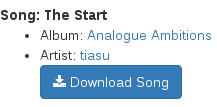
\includegraphics{gfx/search-info}
\newline
Clicking the artist or album, will look up their entries in the \acs{DHT}, and thus
provide detailed information about these. Clicking the 'Download Song' button,
will initialize the download, and add an entry to the download tab, which will
continuously update with information on the download process;

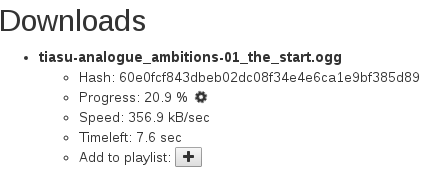
\includegraphics{gfx/download-info}
\newline
{\em It's preferable to use incognito mode, or different browsers for testing this,
as local storage is shared between tab, and may otherwise interfere.}
\newline\newline
Once the content is fully downloaded it'll move to the local tab, from which it
will be seeded and updated with seeding information. 


\includegraphics[width=\linewidth]{gfx/local-info}

\subsection{Playing back content}
The first step is playing back content, is to add the content to the play-list.
This can be done by using clicking one of the small plusses (+), on either the
local content tab, or the download tab.
\newline
After adding a song, one can double-click an entry in the play-list to start the
playback of that entry on the player at the top of the page.

Playing back from the downloads tab (i.e. playing back content, which is
currently downloading), setups the torrent in streaming mode, such that pieces
are download in the order they're needed, rather than in the typical
rarest-first order.
{\em Note that not all file formats can be streamed; streamability and playback
of different file formats is browser dependent, and given by the specific
implementation of the \acs{HTML}5 audio tag.}
\newline\newline
The player contains a variety of buttons, these are considered to be self
explanatory for anyone whom has used a media player before. Below is a full
screen-shot of our web-interface taken while playback of a local song is in
progress.

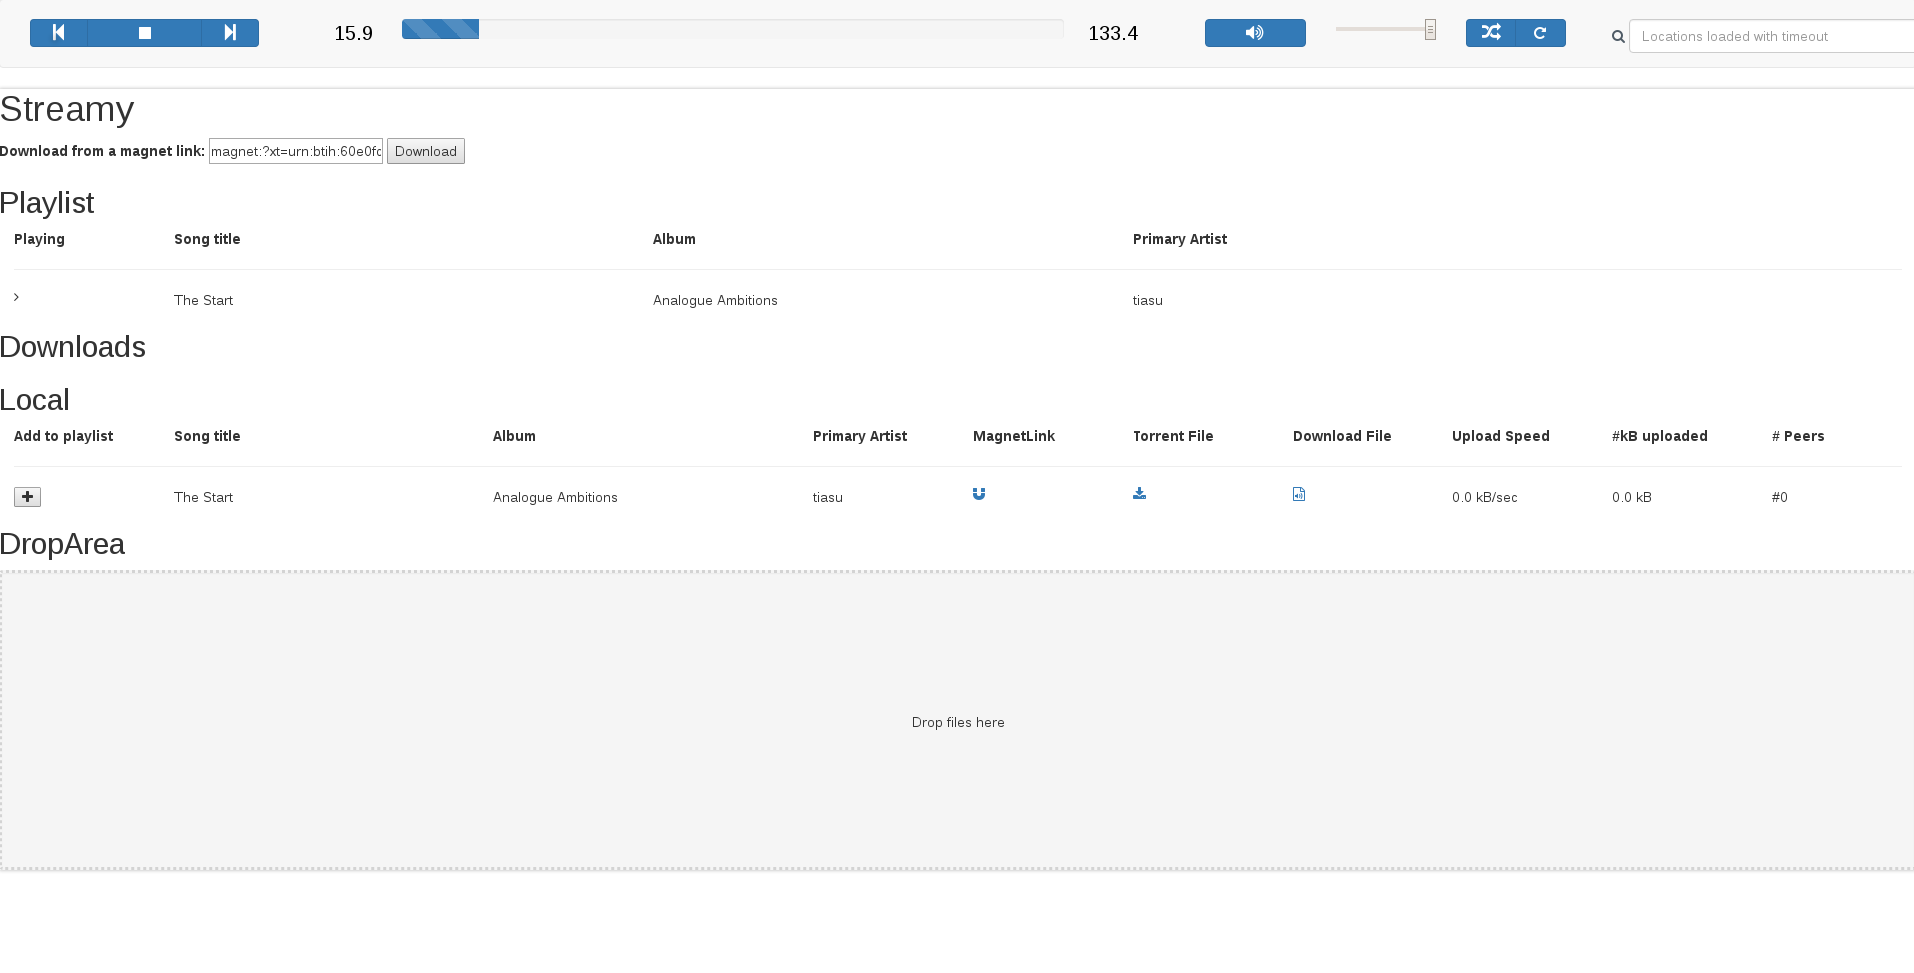
\includegraphics[width=\linewidth]{gfx/interface}
\newline
We encourage the reader to play around with the interface, including with the
features not documented here, such as downloading local-content to disk,
downloading by magnetURI, etc.

\cleardoublepage

\chapter{Showcase}
%\addtocontents{toc}{\protect\clearpage} % <--- just debug stuff, ignore



%\include{multiToC} % <--- just debug stuff, ignore for your documents
% ********************************************************************
% Backmatter
%*******************************************************
\appendix
%\renewcommand{\thechapter}{\alph{chapter}}
\cleardoublepage
\part{Appendix}
\chapter{Contributions}
\label{sec:appendix-contributions}
Throughout the project, we have developed in total 3 sub-projects;
\begin{itemize}
\item Angular2-interface: Our graphic user interface
\item music-streamer-library: A library utilized by our interface
\item fake-dht: A fake implementation of a \acs{DHT} network
\end{itemize}
Below is a list of contributions to each of these projects, by group member;
As the lists contain aliases, we provide a mapping below:
\begin{itemize}
    \item Skeen $\Rightarrow$ Emil Madsen (20105376)
    \item RasmusMJ $\Rightarrow$ Rasmus Mosbech Jensen (20105109)
    \item MortenSoerensen $\Rightarrow$ Morten Kryger Sørensen (20118128)
\end{itemize}

\section{Angular2-interface}
This repository contains our web-interface implemented using Angular2 (also 
known as Angular.io), this interface was developed during the Angular-Attack
hackathon event (May 14-15).
\newline\newline
% TODO: Update LOC
The repository contains 2477 lines of code, at hand-in time, and has undergone 
several refactoring during and after the hackathon.

\begin{figure}[H]
  \centering
    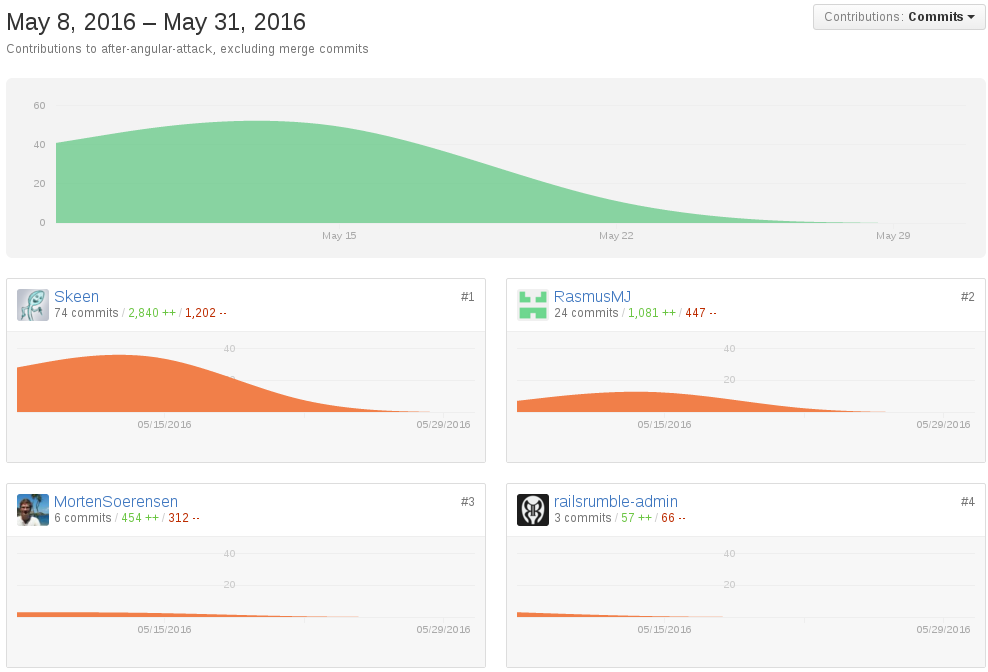
\includegraphics[width=\linewidth]{gfx/Angular-interface}
  \caption{A graph from GitHub laying out contributions by group members. - Angular2-interface}
  \label{fig:angular-interface}
\end{figure}

\section{music-streamer-library}
\label{sec:appendix-music-streamer-library}
This repository contains our library, which underlies our Angular2-interface,
the motivation for splitting the project, is that the library can be utilized 
by multiple interfaces or clients, as we originally intended to develop both a
web-interface client and a node.js client.
\newline\newline
% TODO: Update LOC
To version of the library exists; the stripped version and the unstripped
version. The stripped version contains 949 lines of code, at hand-in time, while
the unstripped version contains 1942 lines of code.

\begin{figure}[H]
  \centering
    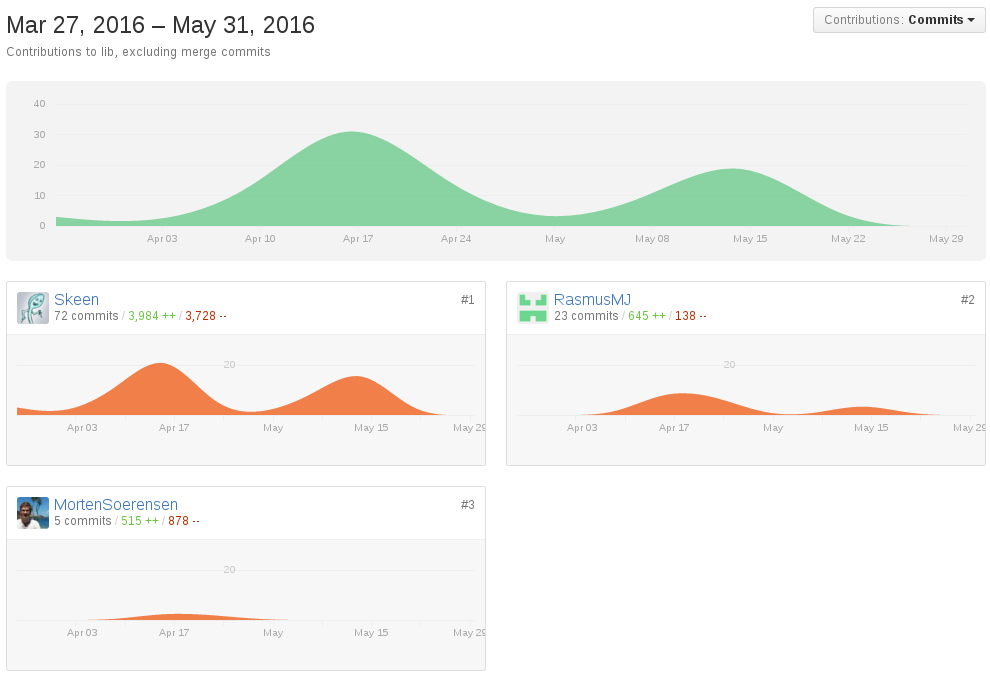
\includegraphics[width=\linewidth]{gfx/Music-streamer-library}
    \caption{A graph from GitHub laying out contributions by group members. - Music-streamer-library (stripped version)}
  \label{fig:music-stramer-library}
\end{figure}

\section{fake-dht}
This repository contains our faked \acs{DHT} implementation, which fulfills the \acs{DHT}
interface within our music-streamer-library by utilizing a centralized server.
\newline
Two different version have been developed, one which fakes a traditional \acs{DHT}
and one which fakes a \acs{PHT} running on top of a \acs{DHT}.
\newline\newline
% TODO: Update LOC
The \acs{DHT} fake contains 101 lines of code, at hand-in time, while the \acs{PHT} fake 
contains 99 lines of code. The two versions utilize different libraries.

\begin{figure}[H]
  \centering
    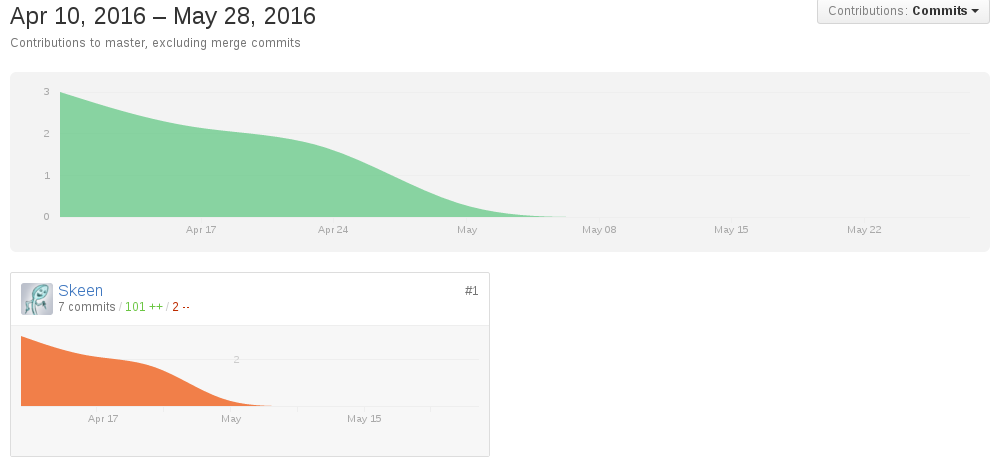
\includegraphics[width=\linewidth]{gfx/dht-fake}
    \caption{A graph from GitHub laying out contributions by group members. - dht-fake}
  \label{fig:music-stramer-library}
\end{figure}

\begin{figure}[H]
  \centering
    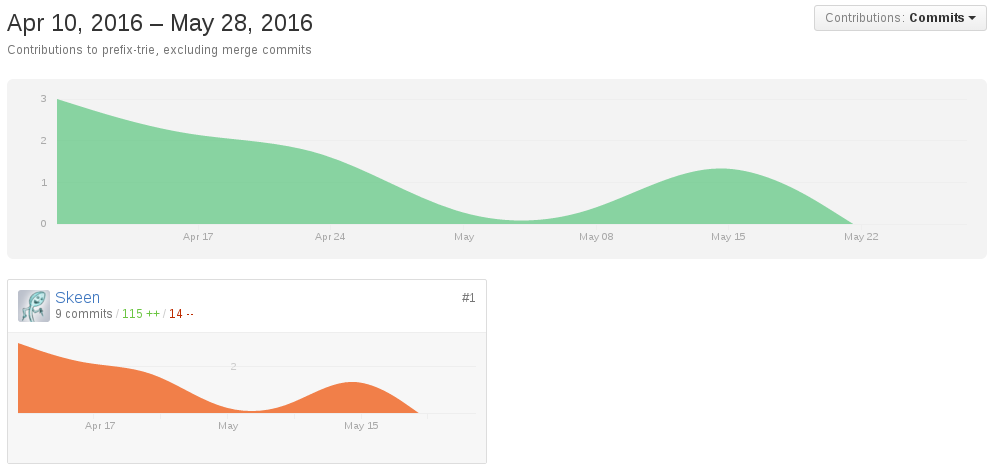
\includegraphics[width=\linewidth]{gfx/pht-fake}
    \caption{A graph from GitHub laying out contributions by group members. - pht-fake}
  \label{fig:music-stramer-library}
\end{figure}

\section{Report}
This section describes the contributions for this very report, which was
written from the 15th of May, till the 1st of June.
\newline\newline
% TODO: Update LOC
%% git ls-files | grep "gfx/" -v | xargs cat | wc -l
The repository contains 3492 lines of code, at hand-in time.

\begin{figure}[H]
  \centering
    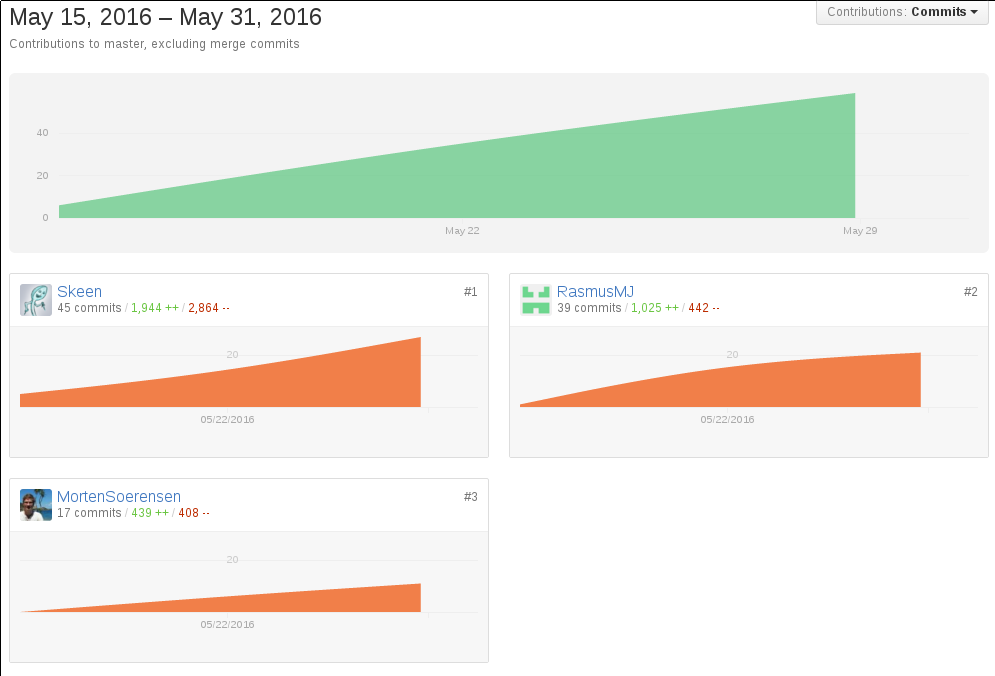
\includegraphics[width=\linewidth]{gfx/report}
    \caption{A graph from GitHub laying out contributions by group members. - report}
  \label{fig:report}
\end{figure}

\section{Other contributions}
In addition to these contributions, we've made several pull requests for the
libraries we depend on; namely to:
\begin{itemize}
\item music-metadata: A library to parse out meta-data from music files.
\item Kad-WebRTC: A transportation layer for the 'Kad' Kademlia implementation.
\item localforage: A unified interface library for persistent browser-storage
    technologies.
\item electron-eval: A library to execute code within a headless browser
    (electron).
\end{itemize}

Below is a list of contributions to each of these projects, by group member:
\subsection{music-metadata}
A pull request and a bug report has been submitted.

\subsubsection{General data stream support}
A \href{https://github.com/leetreveil/musicmetadata/pull/114}{pull request} to
add support for general data streams (not just npm-stream) has been submitted
to the upstream developer: the patch adds 40 lines of code, and removes 40
lines of code.
\newline\newline
The patch was created and submitted by Emil Madsen, and has been rejected by
the upstream developer, whom has implemented the suggested feature in another
way. The newest version of the music-metadata library contains this update.

\subsubsection{Bug report regarding invalid stream usage}
A \href{https://github.com/leetreveil/musicmetadata/pull/116}{pull request} to
add support for stopping read steams as soon as meta-data has been emitted was
accepted into the upstream library.

The content of this pull request did however misuse streams, in a way which is
generally not supported, as such the acceptance of this pull request broke our
code.

Group member Emil Madsen reported this issue to the upstream developer in a
\href{https://github.com/leetreveil/musicmetadata/issues/120}{bug report},
after which the pull request was reverted.

\subsection{Kad-WebRTC}
\label{subsec:appendix-kad-webrtc}
While experimenting with 'Kad-WebRTC' we ran the provided examples, 
unfortunately all of these ran within the same browser tab, and as such we were
not convinced that the library would work across multiple browsers (or tabs).

In order to confirm the operability of the library under these circumstances,
we developed an interactive example, which has been submitted as a 
\href{https://github.com/kadtools/kad-webrtc/pull/11}{pull request}. This pull
request adds 181 lines of code and removes 5.
\newline\newline
The example was created and submitted by Emil Madsen, and has been accepted by
the upstream developer, after a bit of ping-pong regarding the details of the 
pull request.

\subsection{localforage}
\label{subsec:appendix-localforage}
A \href{https://github.com/mozilla/localForage/pull/551}{pull request} to add 
node.js support to the Mozilla project localforage (A unified interface for 
the browser-based persistent storage technologies) has been submitted to the
upstream developers: the patch adds 5664 lines of code (of which 5001 are 
generated by the built system), as such 663 lines of code has been written.
Additionally 3 lines of code has been removed.
\newline\newline
The patch was created and submitted by Emil Madsen, the pull request is still
open, and unlikely to be merged in it's current state. The upstream developers
like the concept and idea presented by the pull request, but cannot accept it,
due to the quality of the utilized libraries.

The created patch do however fulfill our own use-case; that is to enable us to 
develop a proof-of-concept 'node.js' client using our music-streamer-library
(which in turn utilizes localforage for persistent storage).

\subsection{electron-eval}
\label{subsec:appendix-electron-eval}
A \href{https://github.com/mappum/electron-eval/issues/29}{bug report} and 
debugging assistance been provided to the upstream developer, to get the project
running in headless Linux environments (docker for our use-case).
\newline\newline
As a part of this process, several docker images has been created and shared
with the upstream developer, whom has patched the library. This patch combined
with a mapping of the missing external dependencies, has resulted in a
successful recipe for running the project in a headless Linux setting.

The upstream developer considers patching the library further to ease future 
debugging of missing external dependencies. A duplicate of this issue has been
reported to WebTorrent, which was the original blocker for our application.
\newline\newline
The bug report, and the subsequent debugging assistance provided to the
upstream developer was by Emil Madsen.



\chapter{Accepted project proposal}
\label{sec:appendix-project}
%% Project proposal
\centerline{
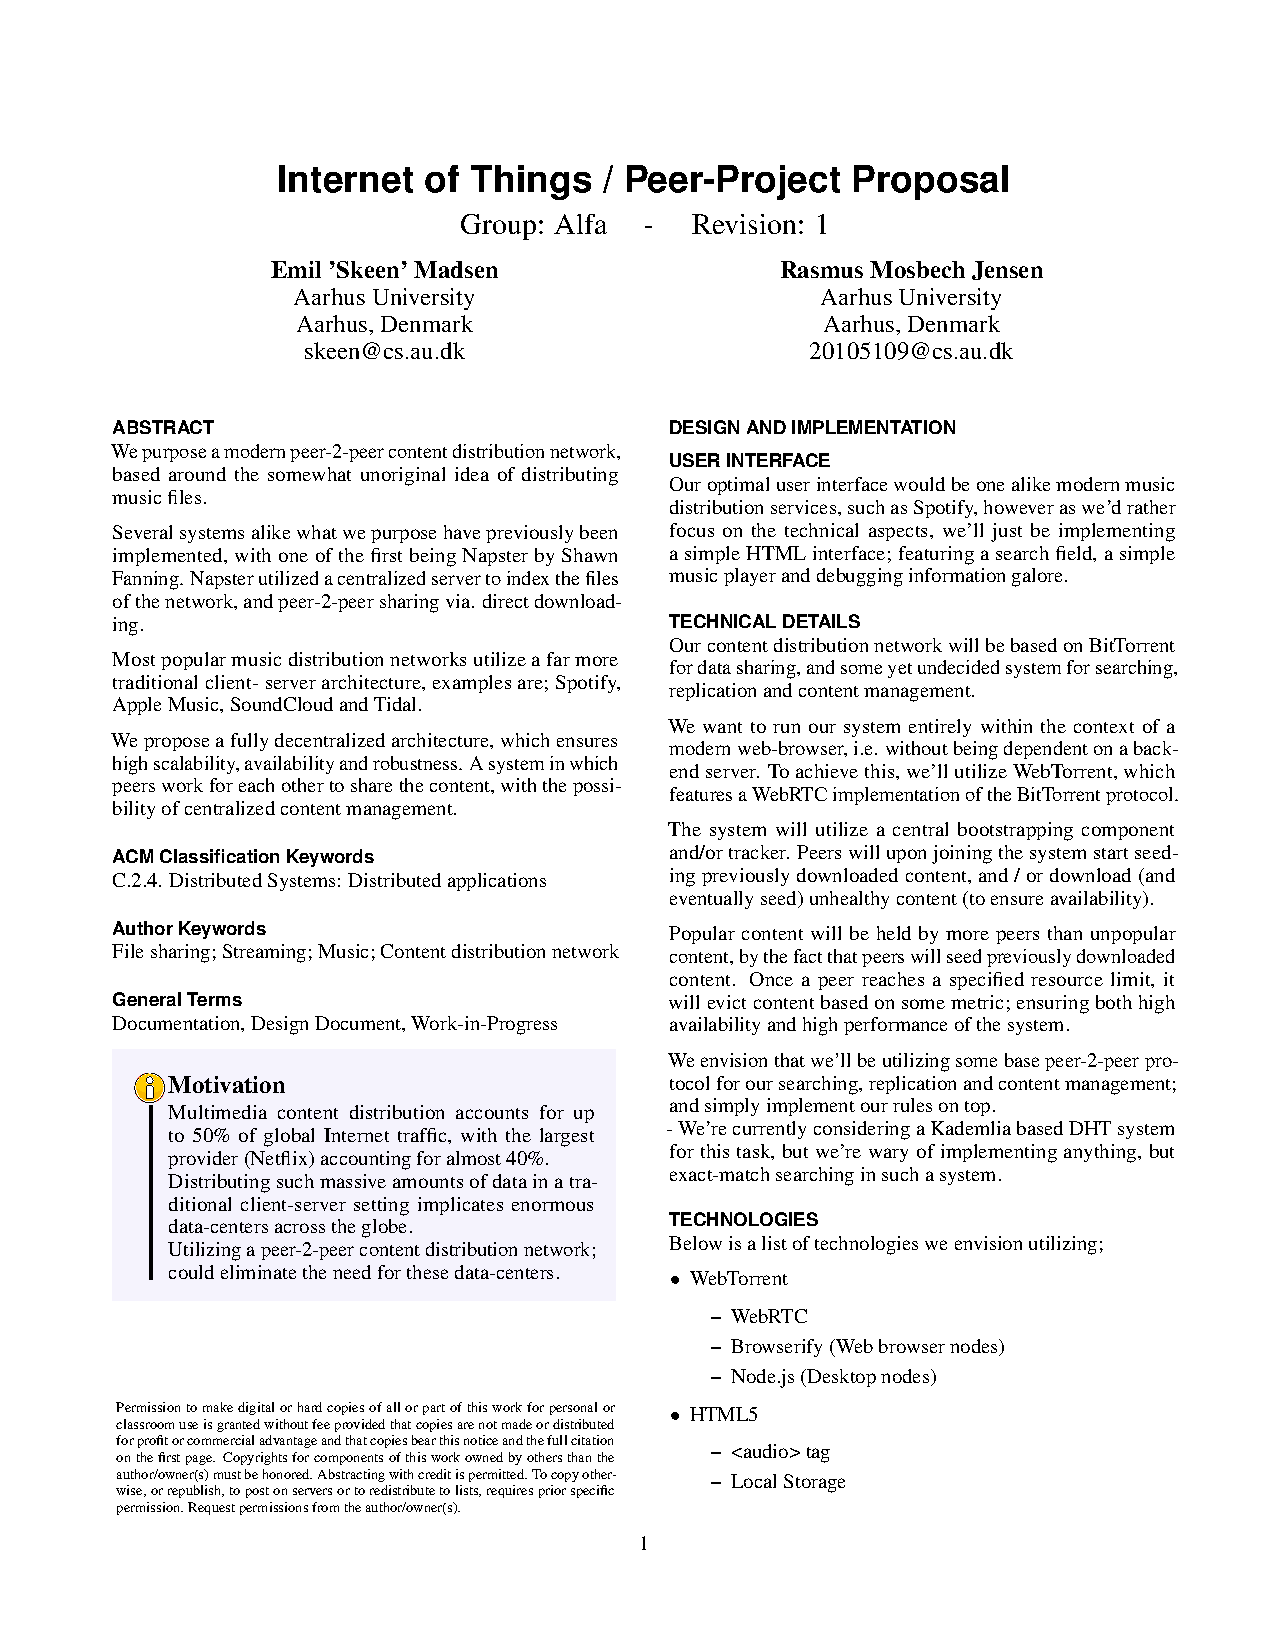
\includegraphics[page=1, scale=0.8]{gfx/project-proposal.pdf}
}

\centerline{
\includegraphics[page=2, scale=0.8]{gfx/project-proposal.pdf}
}


%********************************************************************
% Other Stuff in the Back
%*******************************************************
\cleardoublepage%********************************************************************
% Bibliography
%*******************************************************
% work-around to have small caps also here in the headline
\manualmark
\markboth{\spacedlowsmallcaps{\bibname}}{\spacedlowsmallcaps{\bibname}} % work-around to have small caps also
%\phantomsection 
\refstepcounter{dummy}
\addtocontents{toc}{\protect\vspace{\beforebibskip}} % to have the bib a bit from the rest in the toc
\addcontentsline{toc}{chapter}{\tocEntry{\bibname}}
\label{app:bibliography}
\printbibliography

\cleardoublepage%*******************************************************
% Declaration
%*******************************************************
\refstepcounter{dummy}
\pdfbookmark[0]{Declaration}{declaration}
\chapter*{Declaration}
\thispagestyle{empty}
Put your declaration here.
\bigskip
 
\noindent\textit{\myLocation, \myTime}

\smallskip

\begin{flushright}
    \begin{tabular}{m{5cm}}
        \\ \hline
        \centering\myNameOne \\
    \end{tabular}
\end{flushright}

\begin{flushright}
    \begin{tabular}{m{5cm}}
        \\ \hline
        \centering\myNameTwo \\
    \end{tabular}
\end{flushright}

\begin{flushright}
    \begin{tabular}{m{5cm}}
        \\ \hline
        \centering\myNameThree \\
    \end{tabular}
\end{flushright}

% ********************************************************************
% Game Over: Restore, Restart, or Quit?
%*******************************************************
\end{document}
% ********************************************************************
